% Use the University of Michigan thesis class.
\documentclass[thesis]{thesis-umich}

% Load additional packages
\usepackage{algpseudocode}
\usepackage{algorithm}
\usepackage{array}

% Title of the thesis
\title{Reduced Order Models for Calibration of Nuclear Reactor Simulation Codes}

% Author name
\author{Artem Yankov}

% Department
\department{Nuclear Engineering}

% Year of completion
\year=2013

% Frontispiece
%\frontispiece{\includegraphics[width=4in]{./pics/frontispiece.pdf}}

% Default style for front pages
\frontpagestyle{1}

% Dedication
\dedication{ %
This dissertation is dedicated to...}

% Acknowledgments
\acknowledgments[6]{ %
I would like to thank...}
% This command sets the width of the acknowledgments area as a fraction
% of the total width of the text area.
\acknowledgmentswidth{0.8}

% Committee
\committee{ %
Professor Thomas J. Downar, Chair \\
Professor John C. Lee \\
Professor John P. Boyd}

% Chair must be entered separately for formatting reasons.
\chair{Thomas J. Downar}

% Commands to hide or show lists of figures, tables, etc.
%\hidelistoftables
%\showlistofprograms
%\showlistofappendices

% Definition of any abbreviations used.
\abbreviations{
 \acro{PDE}{partial differential equation}
 \acro{SPDE}{stochastic partial differential equation}
 \acro{HDMR}{high-dimensional model representation}
 \acro{ANOVA}{analysis of variance}
 \acro{TMI}{Three Mile Island}
 \acro{UAM}{Uncertainty Analysis in Modeling}
}

% Some abstract text
\abstract{
Write abstract here!}
%\hideabstractpagenumber

%% DOCUMENT AREA
\begin{document}

% Introduction
\chapter{Introduction}   \label{chap:intro}
% Review of Literature
\section{Overview of Previous Work} 
\label{sec:literature_review}

Modeling nuclear reactor stability and performance computationally has evolved into a multi-physics and multi-scale regime. Various computer codes have been developed and optimized to model individual facets of reactor operation such as neutronics, thermal-hydraulics, and kinetics. These codes are most often coupled to produce more physical results. While it is crucial to be able to produce best-estimate calculations for the design and safety analysis of nuclear reactors, it is equally important to obtain design margins by propagating uncertainty information through the entire computational process. Replacing seemingly arbitrary design margins based on engineering judgement with design margins based on the uncertainty quantification of computer codes can help overcome significant human shortcomings \cite{Eardley}.   

The methodologies used for uncertainty quantification in nuclear engineering have generally mirrored the computational resources available during the time of development. When computational resources were relatively limited, methods based on perturbation theory were derived since the method computation times are independent of the number of input parameters \cite{MLWilliams}. Perturbation theory applies a number of linear approximations and adjoint operators to allow for the retrieval of sensitivity coefficients and basic statistical moments of responses of interest. However, in perturbation theory each desired response requires the solution of a deterministic equation and in some inhomogeneous problems in reactor physics the linear approximations may fail \cite{Gandini}. In addition, application of perturbation theory techniques to computer codes is highly intrusive. Coupled, multiphysics uncertainty analyses using perturbation theory are prohibitive especially when legacy codes are involved. Yet another drawback of perturbation theory in neutronics applications arises in the adjoint-based formulation for cross section uncertainty propagation. In this case, exceptions must be made to responses that cannot be expressed as ratios of reaction rates, as in the transport cross section and \ac{ADFs} \cite{TwoStep_Approach} \cite{Yankov1}. 

As computer resources increased, the linear approximations of perturbation theory were gradually relaxed until routine Monte Carlo sampling became feasible. In the XSUSA method a 44-group covariance matrix is stochastically sampled to generate perturbed few-group cross sections that can be used as input to a Monte Carlo uncertainty analysis in a core simulator \cite{Klein_Gallner}. While uncertainty quantification using Monte Carlo sampling does not apply any approximations to the mathematical system under investigation, the computational expense is tremendous, and the extraction of information such as sensitivity coefficients can be difficult. Nevertheless, sampling provides a brute force means by which many uncertainty quantification algorithms can be validated. 

Recently, an approach based on the stochastic finite element method, referred to as polynomial chaos expansion, has been developed for the purposes of uncertainty quantification \cite{Ghanem_Spanos}. The basic idea behind polynomial chaos expansions is to expand the random variables of some governing stochastic partial differential equations in terms of orthogonal polynomials and then to apply Galerkin projections \cite{LeMaitreKnio}. This idea is similar to the angular expansion of the scatter cross section in terms of Legendre polynomials in neutron transport theory. Methods for uncertainty quantification that employ polynomial chaos expansions fall under the general mathematical framework of spectral methods. The motivation behind spectral methods for uncertainty quantification is to combine the rapid convergence rates of deterministic methods with the generality of stochastic sampling methods. 

While used extensively in structural and materials engineering, polynomial chaos expansions have been seldom applied in nuclear engineering. In \cite{MMR_Williams1} and \cite{MMR_Williams2} the author applies analytic polynomial chaos techniques to investigate the effect of random material properties on radiation transport through a slab in the P1 approximation. The authors in \cite{Ayres_Williams_Eaton} apply non-linear polynomial chaos to examine static and dynamic eigenvalue uncertainties due to uncertainties in cross section values. Finally, the authors in \cite{Fichtl_Prinja} use polynomial chaos-collocation to study the effects of total cross section uncertainties on the probability density function of the scalar flux in absorbing and diffusive media.    

The polynomial chaos expansions based on stochastic galerkin methods applied in the research above exhibit several substantial advantages over Monte Carlo and perturbative methods. Mainly, spectral convergence rates can be achieved. In addition, while nonlinearities and large uncertainties in random variables pose problems for perturbation methods, the stochastic galerkin methods easily deal with such factors. However, the primary drawback of polynomial chaos expansions with stochastic galerkin methods lies in their intrusive nature. In other words, unless an engineering code is initially developed with stochastic galerkin capabilities, which is unlikely, extensive modifications will have to be made to the code. Modifications include adding the ability to solve an enlarged system of coupled, partial differential equations.      

To this end the stochastic collocation method, a variant of polynomial chaos expansion, is considered since it circumvents the need to modify engineering code in order to implement spectrally converging uncertainty quantification methods. Stochastic collocation methods are essentially interpolatory, projecting a set of deterministic simulations onto a polynomial basis. With stochastic collocation codes can be treated as "black boxes". Such an attribute is highly desireable for the uncertainty analysis of nuclear engineering computer codes since often these consist of coupled, multi-physics, and multi-scale legacy code. The success of perturbatory methods, which are linear, in the uncertainty analysis of nuclear engineering codes is indicative of the potential for stochastic collocation. Being a spectral method, stochastic collocation performs best on smooth functions \cite{BoydSpec}.    

However, even when utilizing a stochastic collocation method based on sparse grid constructs, the method suffers from the so-called "curse of dimensionality" \cite{LeMaitreKnio}. The "curse of dimensionality" arises when the convergence of a method is proportional to the exponent of the the function's dimensionality, as in a full tensor product interpolation scheme. While sparse grids help to mitigate the "curse of dimensionality" researchers have shown that when applied to realistic engineering computer simulations the practicality of stochastic collocation diminishes for dimensions greater than $\mathcal{O}(10)$ \cite{AHSGC_HighDimensions}. Consequently, further mitigation is needed in order to apply stochastic collocation to real-world engineering problems. To this end, reduced order models, also known as surrogates and response surfaces, are utilized. Reduced order models work to find a relatively small subspace of some function that is still representative of the original function space. 

Performing uncertainty quantification on high-dimensional, coupled, multiphysics engineering codes can be prohibitive if the codes take many hours to run. To make uncertainty quantification feasible for such problems reduced order models are constructed. While a reduced order model may be computationally expensive to build, the ideal end product is a function that can be evaluated in seconds that captures the behavior of the objective function on which the reduced order model is based.    

%Time to build rom at first, but then pays off for UQ, optimization, inference.
%consequently, reduced order model/surrogate is needed. mathematical surrogate
% discuss paper
% Uncertainty quantification using reduced order models. Stochastic collocation curse of dimensionality, not practical for high dimensions. Must use dimension reduction to make parctical.



 
% Stochastic Partial Differential Equations
\section{Stochastic Partial Differential Equations} \label{sec:spdes}

A \ac{SPDE} is similar in flavor to the better known \ac{PDE}, the main difference being the presence of input uncertainties in the former's parameter space. If the parameters in some \ac{PDE} are probabalistic and the affects of those variable parameters on the outputs are of interest, then the \ac{PDE} must be reforumulated into a \ac{SPDE}. The following example aims to elucidate the difference between \ac{PDE}s and \ac{SPDE}s and to motivate a discussion of the unique features characteristic to \ac{SPDE}s. While these features form the mathematical back-bone for this thesis they are somewhat abstract and not crucial to develping an understanding of the subject matter. 

Consider the \ac{PDE} describing one-speed diffusion of neutron flux in a slab nuclear reactor \cite{Duderstadt}:
% one-speed diffusion theory pde
\begin{eqnarray} \label{eq:one_group_diff_eqn} 
% PDE
   \frac{1}{v} \frac{\partial\phi}{\partial t} 
    - D	\frac{\partial^2\phi}{\partial x^2}
     + \Sigma_{a}\phi(x,t)
      = \nu\Sigma_{f}\phi(x,t) \\
% IC
   \phi(x,0) = \phi_{0}(x) \nonumber \\
% BC
   \phi(a,t) = \phi(-a,t) = 0 \nonumber
\end{eqnarray}
The \ac{PDE} in \ref{eq:one_group_diff_eqn} can be solved for the flux $\phi$ as a function of both space $x$ and time $t$. However, such a solution assumes that the parameters in the \ac{PDE}, namely $v$, $D$, $\Sigma_a$ and $\nu\Sigma_f$, are fixed values. What would happen to the flux if these parameters were described by probability distributions? The flux would be influenced by perturbations to any of the parameters and so the initial two-dimensional problem is converted to a six-dimensional problem, uncertainty in intial and boundary conditions aside. How would the solution to this \ac{SPDE} be found? A few preliminaries are in order.

\subsection{Preliminaries} \label{subsec:SPDEs_prelims}

Most of the language used to describe \ac{SPDE}s comes from the field of probability theory, which is based on the ideas of sets, fields, and events. The notation and definitions described here come mainly from \cite{PrbThryPrlms}. The ultimate purpose of introducing the proceeding ideas from probability theory is to be able to understand random variables and the Doob-Dynkin Lemma. Some of the jargon used to describe sets will also be utilized when discussing dimension-wise function decompositions. A \textit{set} is simply a collection of objects while a \textit{subset} is a collection of objects contained within the larger set. A \textit{sample space} is the set of all outcomes of an experiment and is usually denoted by $\Omega$. For example, if the experiment is flipping a fair coin then the sample space is $\Omega = \left\lbrace	H,T\right\rbrace$. Subsets of $\Omega$ are referred to as \textit{events}. If $\Omega = \left\lbrace\omega_1, \omega_2, ..., \omega_N\right\rbrace$ then the total number of subsets of $\Omega$ is $2^N$, where both the empty set $\emptyset$ and all of $\Omega$ are included in the count.

A few definitions from set algebra are required before moving on to the Doob-Dynkin Lemma. A \textit{union}, or sum, of two sets $A$ and $B$ is the set of elements that are in at least $A$ or $B$ and is denoted by $A\cup B$. The \textit{intersection} of sets $A$ and $B$ consists of all the elements belonging to both $A$ and $B$ and is denoted by $A\cap B$. Finally, the \textit{complement} of a set $A$, denoted by $A^C$, consists of all the elements not in $A$. From these definition, it follows that $A\cup A^C = \Omega$ and $A\cap A^C = \emptyset$.

Now, let's use the ideas of sets, unions, and intersections to define what is meant by a field and sigma field. Let $A$ and $B$ be subsets of the set $\Omega$. The subsets $A$ and $B$ form a \textit{field} $M$ if,
\begin{itemize}
   \item $\emptyset\in M$, $\Omega\in M$
   \item If $A\in M$ and $B\in M$ then $A\cup B\in M$ and $A\cap B\in M$
   \item If $A\in M$ then $A^C\in M$ 
\end{itemize}
A \textit{sigma field} $\mathcal{F}$ is a field that is closed under any countably infinite set of unions and intersections. In other words if subsets $A_1,...,A_n,...$ belong to $\mathcal{F}$ then so do $\bigcup_{i=1}^{\infty} A_i$ and $\bigcap_{i=1}^{\infty} A_i$. Consider the sample space $\Omega= \left\lbrace 1,2,3\right\rbrace$. Following the definition of a sigma field, $\mathcal{F} = \left\lbrace \emptyset, \Omega,\left\lbrace 1\right\rbrace, \left\lbrace 2,3\right\rbrace \right\rbrace$ 
is a sigma field while $\mathcal{G} = \left\lbrace \emptyset,\Omega \left\lbrace2\right\rbrace \right\rbrace$ is not. Rather, the correct sigma field of $\mathcal{G}$ is $\sigma\left(\mathcal{G}\right) = \left\lbrace \emptyset, \Omega, \left\lbrace2\right\rbrace, \left\lbrace 1,3\right\rbrace\right\rbrace$. The notation $\sigma\left(\mathcal{U}\right)$ is used to denote the smallest sigma field containing $\mathcal{U}$, where $\mathcal{U}$ is a collection of subsets of $\Omega$. In general, such a sigma field can be constructed by,
% Construction of sigma algebra
\begin{equation} \label{eq:construct_sigma_algebra}
   \sigma\left(\mathcal{U}\right) = \bigcap_{\mathcal{A}}
     \left\lbrace \mathcal{U} \subset \mathcal{A} 
     \textrm{:} \mathcal{A} \textrm{ is a sigma field} \right\rbrace 
\end{equation}        
A \textit{Borel sigma algebra} is $\mathcal{B} = \sigma\left( \mathcal{U}\right)$ where $\mathcal{U}$ consists of all the open sets in $\mathbb{R}^N$.

Combining the ideas described above, a \textit{probability space} $\left(\Omega,\mathcal{F},P \right)$ consists of a sample space $\Omega$, a sigma field $\mathcal{F}$ of subsets of $\Omega$, and a probability function $P$ on $\left(\Omega,\mathcal{F}\right)$. The probability function must satisfy the three axioms of probability, which are given as:
\begin{enumerate}
   \item $P(A)\geq 0$
   \item $P\left(\Omega\right)=1$
   \item $P\left(A\cup B\right)=P\left(A\right)+P\left(B\right)$ if
      $A\cap B=\emptyset$
\end{enumerate} 
An example will help make some of these abstract concepts more concrete. Consider the experiment of tossing a fair coin. The sample space is $\Omega =\left\lbrace H,T\right\rbrace$  and the sigma field of events is  $\mathcal{F}=\left\{\left\{H\right\},\left\{T\right\}, \Omega,\emptyset\right\}$. Probabilities of events in $\mathcal{F}$ are $P\left({H}\right) = P\left({T}\right)=1/2$, $P\left(\Omega\right) = 1$ and $P\left(\emptyset\right) = 0$.

At this point, enough background has been given to describe a \textit{random variable} in general terms. Uncertainty quantification pioneer Gianluca Iaccarino writes, "Random variables are the building blocks for studying uncertainties in a probabilistic framework" \cite{Iaccarino_quote}. In the simplest terms, a random variable takes events and assigns them a real number. Let $X$ be a random variable. Then $X$ takes an event $\omega$ from the event space $\Omega$ and maps it to a number on the real line $X\left(\omega\right): \Omega \rightarrow \mathbb{R}$. Under such a mapping a whole region $A_B \in \Omega$ gets mapped to an interval $B$ on the real line. A more formal definition of a random variable can be made using the language of set theory. Let $\left(\Omega,\mathcal{F},P\right)$ be a probability space. A mapping $X:\Omega \rightarrow \mathbb{R}^N$ measurable with respect to $\mathcal{F}$ is a random variable. In other words, for any open set $A$ in $\mathbb{R}^N$, $X^{-1}\left(A\right) \in \mathcal{F}$ is a random variable.

As an example, consider the event space $\Omega=\left\{1,2,3\right\}$ and the sigma field \ $\mathcal{F}=\left\{\emptyset, \Omega, \left\{1\right\}, \left\{2,3\right\}\right\}$. Then if we define $Y\left(1\right)=1$, $Y\left(2\right)=0$, and $Y\left(3\right)=-1$ then $Y$ is not a random variable because $\left\{3\right\}\notin \mathcal{F}$. Now, if we define $Z\left(1\right)=1$, and $Z\left(2\right)=Z\left(3\right)=0$ then $Z$ is a random variable because $\left\{1\right\}$ and $\left\{2,3\right\}$ are both in $\mathcal{F}$. This example serves to demonsrate the interconnectedness between  sigma fields and event spaces.

The purpose of the preceeding discussion was to build a sufficient framework to be able to state the Doob-Dynkin lemma. Let $X:\Omega \rightarrow \mathbb{R}^N$ be a random variable and let $\mathcal{B}$ be the Borel sigma algebra. The sigma algebra generated by $X$ is $\sigma\left(X\right)=\left\{X^{-1}\left(F\right):F\in\mathcal{B}\right\}$. The Doob-Dynkin lemma describes the relationship between a random variable and the sigma field it generates. Let $X,Y:\Omega \rightarrow \mathbb{R}^N$ be two functions. Then $Y$ is $\sigma\left(X\right)$ measurable if and only if there exists a Borel measurable function $g:\mathbb{R}^N \rightarrow \mathbb{R}^N$ (for any $A\in \mathcal{B},g^{-1}\left(A\right)\in\mathcal{B}$) such that $Y=g(X)$. To say that $Y$ is "$\sigma\left(X\right)$ measurable" means that if $X$ is known then  $Y$ is known as well \cite{PrbThryPrlms}. When a \ac{PDE} is transformed into a \ac{SPDE} by treating the parameters as random variables it is appropriate to question whether the solution of the \ac{SPDE} can be described in terms of the same random variables \cite{AHSGC}. The Doob-Dynkin lemma answers this question with a resounding yes.
          
\subsection{Application to Engineering Systems} \label{subsec:spde_apps2engineering} 
 
In this section, the theory of \ac{SPDE}s is applied to the types of problems that typically arise in nuclear engineering. Much of the notation used in the proceeding discussion is borrowed from \cite{KarLoeXiu}. First, define the physical domain as $\mathcal{D} \subset \mathbb{R}^{d}$ where $d$ can be $1$, $2$, or $3$ depending on the number of spatial dimensions being considered. The boundary of the domain is designated as $\partial\mathcal{D}$. Any coordinate living in the spatial domain can be described by some vector $\textbf{x}=\left(x_1,...,x_d\right)$. The most general mathematical systems that are of interest can be written as,
% General PDEs with random parameters we are trying to solve
\begin{eqnarray} 
\label{eq:pde_general1}
% domain
    \mathcal{L}\left(\textbf{x},\omega;u\right)=f\left(\textbf{x},\omega\right)
        \hspace{1 cm} \textbf{x} \in \mathcal{D}  \\
\label{eq:pde_general2}    \mathcal{B}\left(\textbf{x};u\right)=g\left(\textbf{x}\right) 
        \hspace{1 cm} \textbf{x} \in \partial\mathcal{D}.
\end{eqnarray}
Ultimately, $u:\Omega \times \mathcal{D}\rightarrow \mathbb{R}$ is sought after since $u$ is the solution to \ref{eq:pde_general1} and \ref{eq:pde_general2}, where $\mathcal{L}$ is a linear/non-linear differential operator, $\mathcal{B}$ is a boundary operator, and $f$ and $g$ are driving terms. The system in \ref{eq:pde_general1} and \ref{eq:pde_general2} is defined over a complete probability space $\left(\Omega,\mathcal{F},P\right)$ with $\omega \in \Omega$, as defined previously. Of course, \ref{eq:pde_general1} and \ref{eq:pde_general2} must be well-posed in the sense of Hadamard \cite{Hadamard}. In Hadamard's definition, well-posed mathematical models of physical phenomena satisfy three conditions:
\begin{enumerate}
    \item Existence of a solution
    \item Uniqueness of the solution
    \item The solution is not sensitive to small perturbations in initial conditions 
\end{enumerate} 
Generally, well-posed problems can be solved using stable computer algorithms. However, it is important not to confuse posedness with conditioning as the two describe very different things. Problems that are typically not well-posed, such as inverse problems, can be formulated as well-posed problems through regularization.     

The problem in \ref{eq:pde_general1} and \ref{eq:pde_general2} is continuous and as such, will not have an analytic solution for practical problems in engineering applications. An infinite number of random variables are needed to fully describe the stochastic process. Since modeling such a process on a computer is impossible, the infinite-dimensional probability space must be reduced to a finite-dimensional space. The procedure to do this is referred to as the "finite-dimensional noise assumption". The Karhunen-Loeve expansion of the stochastic space achieves this reduction in dimensionality with the benefit of being able to fully model the full stochastic space if desired \cite{KarLoeXiu}.

Applying the Karhunen-Loeve expansion to \ref{eq:pde_general1}, the random inputs can be characterized by a set of $N$ random variables as,
\begin{equation} \label{eq:rand_pde_general}
    \mathcal{L}\left(\textbf{x},Y_{1}(\omega),...,Y_{N}(\omega);u\right) = 
     f\left(\textbf{x},Y_{1}(\omega),...,Y_{N}(\omega)\right)
\end{equation}
where $\left\{Y_i(\omega)\right\}_{i=1}^N$ are uncorrelated random variables. By the Doob-Dynkin lemma, the solution of \ref{eq:pde_general1} and \ref{eq:pde_general2} can be expressed in terms of the same random variables $\left\{Y_i(\omega)\right\}_{i=1}^N$. Hence, the solution to the \ac{SPDE} can be written as $u\left(\textbf{x},\omega\right)=u\left(\textbf{x},Y_{1}(\omega),...,Y_{N}(\omega)\right)$. Equations \ref{eq:pde_general1} and \ref{eq:pde_general2} with a discrete stochastic space can be restated as, 
% SPDEs with discrte stochastic space
\begin{eqnarray}
\label{eq:rand_pde_general1}
    \mathcal{L}\left(\textbf{x},\textbf{Y};u\right) = 
     f\left(\textbf{x},\textbf{Y}\right) \hspace{1 cm} \left(\textbf{x},
      \textbf{Y}\right)\in D \times \Gamma \\
\label{eq:rand_pde_general2}
    \mathcal{B}\left(\textbf{x},\textbf{Y};u\right) = 
     g\left(\textbf{x},\textbf{Y}\right) \hspace{1 cm} \left(\textbf{x}, 
      \textbf{Y}\right)\in \partial D \times \Gamma 
\end{eqnarray} 
where $\Gamma_i$ is the image of the independent random variables $Y_i\left(\omega\right)$. Without loss of generality $\Gamma_i$ can be restricted to $\left[0,1\right]$ for $i=1,...,N$. Consequently, the bounded stochastic space, or support, is an $N$-hypercube $\Gamma=\left[0,1\right]^N$. No limits have really been imposed on the stochastic space since any bounded region can be mapped to the unit hypercube. In \ref{eq:rand_pde_general1} and \ref{eq:rand_pde_general2} what remains is a set of independent, deterministic equations in space that can be solved using any deterministic discretization technique. The stochastic problem has essentialy been decoupled from the spatial problem.          

% Uncertainties in Nuclear Data
\section{Uncertainties in Nuclear Data}
\label{sec:cross_sec_uncertainties}

\subsection{Cross Section Uncertainty Overview}
\label{subsec:xsec_uq_overview}

While the methods described in this thesis are applicable to a plethora of engineering applications, the target application here concerns the simulation of nuclear reactors. A main component of any reactor analysis is a description of the neutronics, the physical processes behind neutron transport inside a reactor. When studying uncertainty quantification and sensitivity analysis of the neutronics in some reactor system, the primary  player has been shown to be uncertainty in cross section data \cite{Khalik_Turinsky} \cite{Jessee_Khalik_Turinsky}. Cross section uncertainties for various reactions, energies, and nuclides are accumulated during their experimental determination. Many of the cross sections exhibit correlations among themselves that must be taken into account. A problem arises when one becomes interested in performing uncertainty and sensitivity analysis on a core simulator since the simulators use processed cross section data. The experimental cross section uncertainties and covariances must be carefully propagated down through the standard cross section processing regime.   

Until recently, the primary approach for cross section uncertainty propagation involved the application of first-order perturbation theory. The perturbation theory approach is described in detail in \cite{MLWilliams}. Basically, for neutronics uncertainty analysis this approach entails the solution of an adjoint transport equation for each response of interest, allowing for the efficient retrieval of sensitivity coefficients for all input data. The sensitivity coefficients can then be used to obtain response uncertainties by being operated on by the inputs' covariance matrix. However, the linear approximations in perturbation theory and generalized perturbation theory may fail in certain scenarios. In particular, if the ratio of neutron loss due to absorption is high, such as when a control rod is rapidly inserted, second order effects may become substantial \cite{MLWilliams}. In addition, while perturbation theory may be computationally efficient for problems where only a handful of responses are of interest, problems with many responses may be burdensome due to the need to solve the generalized adjoint transport equation for each response. Not to mention, implementation of the perturbation theory approach is intrusive to engineering codes which makes uncertainty quantification of coupled, multiphysics code systems  infeasible.         

With the recent increase in accessibility to parallel computing environments stochastic sampling methods have become popular since they do not apply any kind of approximations to the physics at hand. Consequently, for cross section uncertainty propagation sampling methods have also been adopted to replace perturbation theory. A description of the process for propagating experimental uncertainties in cross section data to few group cross sections is described in this section. The statistical sampling framework for cross section data is extremely flexible since uncertainties can be calculated for any few group parameters. The same cannot be said of perturbation theory, which must formulate responses as ratios of reaction rates. Consequently, uncertainties for few group transport cross sections and assembly discontinuity factors are difficult to obtain using generalized perturbation theory.   

\subsection{Sampling Method}
\label{subsec:xsec_sampling}

The method for producing stochastically sampled few-group cross sections will be described. Although the method described is quite general, to provide clarity it will be described in the context of the \ac{SCALE} code \cite{SCALE}. Specifically, \ac{SCALE}'s \ac{ENDF} libraries and cross section processing utilities will be detailed. In the \ac{ENDF} libraries the multigroup cross sections are assumed to be Gaussian and consequently, they can be fully characterized by their means and covariances. The \ac{SCALE} 44-group \ac{ENDF}/B-VII covariance matrix contains generic multigroup covariance data. For a problem where $m$ nuclide-reaction combinations are of interest the pertinent covariance matrix is expanded to a size of $\left[m\cdot 44\right]\times \left[m\cdot 44\right]$. The Gaussian assumption imposed on the cross section values implies the cross sections can take on negative values. Since cross sections physically cannot take on negative values their distributions are truncated \cite{Klein_Gallner}.      

The first step towards obtaining perturbed few-group cross sections is to sample the generic multigroup covariance library. The covariance data schema in \ac{SCALE} is given as relative values of infinitely dilute cross sections \cite{Williams_Ilas}. Denote the 1D energy dependent, pointwise cross section for reaction $x$ as $\sigma_x(E)$. The infinitely dilute cross section in energy group $g$ can then be calculated as,
\begin{equation}
\label{eq:infinitely_dilute_xsec}
   \sigma_{x,g}(\infty) = \frac{\langle\sigma_x(E)\rangle}
    {\Delta u_g}   
\end{equation}  
where the bracket notation indicates a lethargy inner product over the energy interval covered by group $g$. Consequently, when the multigroup covariance matrix in \ac{SCALE} is sampled the resulting perturbation $\sigma_{x,g}'$ to the infinitely dilute cross sections can be expressed in terms of a perturbation factor $Q_{x,g}$,
\begin{eqnarray}
\label{eq:infinitely_dilute_xsec_prime}
   \sigma_{x,g}'(\infty) &=& \left(1 + \frac{\Delta\sigma_{x,g}(\infty)}
    {\sigma_{x,g}(\infty)}\right)\sigma_{x,g}(\infty) \nonumber \\
     \nonumber \\
      &=& Q_{x,g}\sigma_{x,g}(\infty). 
\end{eqnarray}  
The perturbations in Eq. \ref{eq:infinitely_dilute_xsec_prime} will provide generic multigroup cross section values to propagate through a transport solver, which can then yield perturbed few-group cross section values. However, to make the perturbed cross sections problem specific they must undergo adjustments due to resonance self shielding. For this purpose, perturbed pointwise cross sections and perturbed Bondarenko self-shielding factors are required. The pointwise, or continuous energy, cross sections are needed to perform 1D transport calculations in the resolved resonance range while the Bondarenko factors are applicable in the unresolved energy range. Since the pointwise cross sections, Bondarenko factors, and generic infinitely dilute multigroup cross section are related algebraically it is necessary to perturb each in terms of the factor $Q_{x,g}$. 

In \cite{Williams_Ilas} the authors show that, given a perturbation factor $Q_{x,g}$, the appropriate pointwise cross sections perturbation can be obtained by,
\begin{equation}
\label{eq:pointwise_xsec_prime}
   \sigma_x'(E) = Q_{x,g}\sigma_x(E) \hspace{1cm} E\in g.
\end{equation} 
From Eq. \ref{eq:pointwise_xsec_prime} it is clear that the pointwise cross section data gets perturbed uniformly in a given energy group $g$, which is a valid approximation if the energy width is small. The authors in \cite{Williams_Ilas} note that although this approximation leads to discontinuities at the energy group boundaries, it does not impact the resulting multigroup data significantly. No significant impact is expected because the multigroup data is averaged using fluxes and cross sections from the same energy bin. 

At this point, infinitely dilute multigroup cross sections and pointwise cross sections can be consistently perturbed using the \ac{SCALE} \ac{ENDF} covariance library. To proceed with a transport calculation using perturbed parameters, perturbed Bondarenko self-shielding factors $f_{x,g}'(\sigma_0)$ are also needed. The Bondarenko factors are expressed in terms of the background cross section $\sigma_0$, pointwise cross sections, and infinitely dilute cross sections as,     
\begin{equation}
\label{eq:bondarenko}
   f_{x,g}(\sigma_0) = \frac{1}{\sigma_{x,g}(\infty)}
    \Big\langle \frac{\sigma_x(E)}{\sigma_t(E) + \sigma_0}\Big\rangle
     \Big/
     \Big\langle \frac{1}{\sigma_t(E) + \sigma_0}\Big\rangle.
\end{equation}
Substituting Eqs. \ref{eq:infinitely_dilute_xsec_prime} and \ref{eq:pointwise_xsec_prime} into Eq. \ref{eq:bondarenko}, the perturbed Bondarenko factor is obtained,
\begin{equation}
\label{eq:bondarenko_prime}
   f_{x,g}'(\sigma_0) = \frac{1}{Q_{x,g}\sigma_{x,g}(\infty)}
    \Big\langle \frac{Q_{x,g}\sigma_x(E)}{Q_{t,g}\sigma_t(E)+\sigma_0}\Big\rangle
     \Big/
     \Big\langle \frac{1}{Q_{t,g}\sigma_t(E) + \sigma_0}\Big\rangle.
\end{equation}
The authors in \cite{Williams_Ilas} show that Eq. \ref{eq:bondarenko_prime} can be evaluated by simply evaluating the unperturbed Bondarenko equation in Eq. 
\ref{eq:bondarenko} at a perturbed background cross section $\sigma_0' = \sigma_0/ Q_{t,g}$. Note that only those cross sections whose uncertainties are specified in the \ac{SCALE} covariance library can be processed and propagated through transport calculations. Since covariance data for 2D scattering distributions is not available in the \ac{SCALE} \ac{ENDF}/B-VII covariance library, their uncertainty affects cannot be quantified in any analyses \cite{Williams_Ilas}. 
 
\subsection{Cross Section Sampling in SCALE}
\label{subsec:scale_sampler}  

The method described in section \ref{subsec:xsec_sampling} for producing perturbed cross sections will be further described in the context of the modules in \ac{SCALE}. The first step is to produce perturbation factors using the module XSUSA by sampling the \ac{SCALE} \ac{ENDF}/B-VII covariance library. If a total of $N_1$ output files of transport solver are desired then $N_1$ sets of perturbation factors are to be obtained. Using the perturbation factors, the \ac{SCALE} module CLAROL+ yields perturbed, infinitely dilute, multigroup cross sections by essentially applying Eq. \ref{eq:infinitely_dilute_xsec_prime}. The resulting cross sections are then passed to the module CRAWDAD+, which outputs perturbed, continuous energy cross sections. To make the multigroup cross sections problem specific they are passed to the BONAMI module, which adjusts the cross sections to account for self-shielding effects in the unresolved energy region using the Bondarenko shielding factor method. Perturbed Bondarenko factors are used in BONAMI, as output from CLAROL+ upon application of Eq. \ref{eq:bondarenko_prime}.

At this point the cross sections still need to be processed for self-shielding effects in the resolved energy region. The \ac{SCALE} modules CENTRM/PMC are responsible for folding in these effects into the multigroup cross sections. CENTRM solves the neutron slowing down equation on an ultra fine spectra on the order of $\mathcal{O}(10^4)$ energy points. For the flux a linear interpolation scheme is used between energy points to produce a continuous energy solution over the entire energy range \cite{Williams_Gehin}. The CENTRM module incorporates actual composition, temperature, and environment dependent effects into the resonance shielded cross sections. PMC accepts the high resolution flux spectra output by CENTRM and averages pointwise nuclear data into multigroup cross sections, which are now tailored to solve the specific problem of interest.              

Finally, the problem specific multigroup cross sections output by CENTRM/PMC are sent to a lattice transport solver, which in this case is the \ac{SCALE} module NEWT. In general, NEWT can be replaced by any transport solver. However, for the purposes of producing few group cross sections a lattice transport solver will generate the multigroup flux distribution for some heterogeneous configuration, which is then used to generate homogenized few group cross sections and intra-assembly flux shapes. A script to extract desirable output quantities from the transport output, such as few group cross sections and kinetics parameters, is needed. Such a script is executed after each of $N_1$ calls to NEWT. Each call extracts a set of perturbed, few group cross sections that are ultimately propagated through a core simulator. The SAMPLER sequence in \ac{SCALE} automates the process of producing perturbed cross section sets \cite{Williams_Ilas}.      

With the availability of $N_1$ perturbed few group cross section sets, each set containing all the nuclear data required by a core simulator, the sets can be directly propagated through the core simulator. The desired results from each simulation can then be gathered and statistically analyzed in what is referred to as the 'one-step' method. However, in what is referred to as the 'two-step' method, the $N_1$ perturbed few group cross section sets can be used to create a few group covariance matrix \cite{TwoStep_Approach}. The few group covariance matrix is then sampled and each sample is propagated through the core simulator. Both the 'one-step' and 'two-step' methods have been shown to produce consistent results \cite{TwoStep_Approach}. However, the 'two-step' method has the advantage of breaking the limitation on the number of samples that can be propagated through the core simulator. In the 'one-step' method each core simulation requires a corresponding transport solution. Transport solutions are relatively expensive to compute when compared to core simulations. A flow diagram of the 'two-step' method is displayed in Figure \ref{fig:sampler_flow_diagram}. For the 'one-step' method $N_1=N_2$ whereas for the 'two-step' method $N_2 >> N_1$, allowing for the acquisition of better statistics.        
\begin{figure}
\caption['Two-Step' method flow diagram.]{\label{fig:sampler_flow_diagram}
Flow diagram of 'two-step' method for core simulators.}
\begin{tikzpicture}[node distance = 3.5cm, auto]
\tikzstyle{every node}=[font=\small]
   % Place nodes
   \node [block1] (xsusa) {\textbf{XSUSA}: Make random perturbations to covariance 
   library};
   \node [block, below of=xsusa] (clarol) {\textbf{CLAROL+}: 
   Perturb MG xsecs and shielding factors};
   \node [block, below of=clarol] (crawdad) {\textbf{CRAWDAD+}: 
   Perturb CE xsecs};
   \node [block, right of=clarol, node distance=8cm] (bonami) {\textbf{BONAMI}: 
   Perform self-shielding calculations in unresolved energy region};
   \node [block, right of=crawdad, node distance=8cm] (centrm) 
   {\textbf{CENTRM/PMC}: 
   Perform self-shielding calculations in resolved energy region};  
   \node [block, below of=centrm] (newt) {\textbf{NEWT}: 
   Perform transport calculations using perturbed xsecs};
   % Invisible nodes
   \node [left of= xsusa, node distance=2.5cm, scale=0.01] (xsusa_i) {};
   \node [left of= newt, node distance=4.5cm, scale=0.05] (newt_l) {};
   \node [block, below of=newt_l, node distance=3.0cm] (cov) {Sample 
   $C_{\Sigma_{FG}}$ matrix};
   \node [block, below of=cov] (core) {\textbf{Core Simulator}: Simulate perturbed
   input data};
   % Invisible npde
   \node [left of= cov, node distance=6.0cm, scale=0.05] (cov_i) {};
   \node [left of= core, node distance=3.5cm, scale=0.05] (core_i) {};
   \node [block1, below of=core_i, node distance=3.0cm] (stats) {Analyze $N_2$ 
   results};
   
   % Draw edges
   \path [line] (xsusa) -- node (xsusa_o) {$Q_{x,g}$} (clarol);
   \path [line] (clarol) -- (crawdad);   
   \path [line] (clarol) -- node (clarol_o) {$\sigma_{x,g}'(\infty)$, 
   $f_{x,g}'(\sigma_0)$} (bonami);
   \path [line] (crawdad) -- node (crawdad_o) {$\sigma_{x}'(E)$} (centrm);
   \path [line] (bonami) -- node[left] (bonami_o) {initial self-shielded data}
   (centrm);
   \path [line] (centrm) -- node[left] (centrm_o) {final self-shielded data} 
   (newt); 
   \path [-,draw] (newt) -| node[below]{Repeat $N_1$ times} (xsusa_i.north);
   \path [line]{} (xsusa_i.north) |- node{} (xsusa);  
   \path [line] (newt_l) -- node[left] (newt_lo){$C_{\Sigma_{FG}} =$ Cov 
   $(\Sigma_{FG_1}...\Sigma_{FG_{N_1}})$} (cov);
   \path [line] (cov) -- node[left] (cov_o){$\Sigma_{FG_i}'$} (core); 
   \path [-,draw] (core) -| node[below]{Repeat $N_2$ times} (cov_i.north);
   \path [line]{} (cov_i.north) |- node{} (cov);
   \path [line] (core_i) -- (stats); 
\end{tikzpicture}   
\end{figure}



  



% NEED CHAPTER ON OVERVIEW OF CURRENT UQ METHODS IN REACTOR ANALYSIS

% Reduced Order Models
\chapter{Reduced Order Models for Computer Codes} \label{chap:rom}
% Reduced-Order Models

Computer codes that model physical phenomena typically accept an input file whose purpose is to describe specific conditions in the universe being modeled by the code. The code is executed and the affects of the conditions on some dependent quantities are output. From this perspective computer codes can be viewed and treated in much the same way functions mathematicians deal with are treated. Like matrices, functions with certain properties can undergo various decompositions that offer insight into their structure. The purpose of \ref{sec:func_decomp} is to describe a technique for decomposing functions into orthogonal components, with the ultimate intention of applying the technique to computer codes. It is hoped that the decomposition of the computer code in terms of its inputs reveals which inputs play the most active roles in the underlying physics. Keeping only the most active dimensions in the decomposition, a reduced order model is effectively built. However, the function decomposition technique described in \ref{sec:func_decomp} describes only half the story. To create a reduced order model of a computer code that can be efficiently evaluated at any state point in the original parameter space an efficient, multidimensional, interpolation scheme is needed. Such a scheme is discussed in \ref{sec:smolyak_sg}. The coupling between interpolation and function decomposition that creates a usable reduced order model is described in \ref{sec:decomp_and_interp}.    

% Function Decompositions
\section{Function Decompositions} \label{sec:func_decomp}

In order to reduce the dimensionality of some function there must exist a metric to determine the importance of each dimension with respect to the others. It's important to have a framework that isolates the effects of each dimension on the output of the function. The framework chosen to perform dimension reduction is formally known as \ac{HDMR}. In statistics, the \ac{ANOVA} decomposition is a special case of \ac{HDMR} where the Lebesgue measure is used to perform all integrations.

\subsection{Dimension-wise Decompositions} \label{subsec:dim_wise_decomps}

The dimension-wise \ac{HDMR} is algorithmically similar to Gram-Schmidt for matrix orthogonalization in that orthogonal components are systemically removed to create a linearly independent basis. As in Gram-Schmidt, the essential operator in dimension-wise \ac{HDMR} is the projection operator. Before introducing the projection operator of interest in this thesis, define the $d$-dimensional product measure to be,
\begin{equation} \label{eq:d_dimension_product_measure}
    d\mu\left(\textbf{x}\right) = \prod_{j=1}^{d}
                              d\mu_{j}\left(x_j\right) 
\end{equation}
where $\mu_j$ are probability measures defined over some $\Omega$. Two functions $f,g:\Omega^d \rightarrow \mathbb{R}$ are considered orthogonal with respect to the product measure defined in \ref{eq:d_dimension_product_measure} if the inner product,
\begin{equation} \label{eq:inner_product}
   \left(f,g\right)=\int_{\Omega^d} f(\textbf{x})g(\textbf{x})d\mu(\textbf{x})
\end{equation} 
is equal to zero. To introduce the projection operator $P_\textbf{u}$, the notation used in \cite{Holtz} is adopted. The operator $P_\textbf{u}$ projects from a $d$-dimensional space to a $\vert\textbf{u}\vert$-dimensional space for some set $\textbf{u}\subseteq \mathcal{D}$, where $\mathcal{D}=\lbrace 1,...,d\rbrace$ consists of the set of all coordinate indices in $\textbf{x}$. The projection on to $\textbf{u}$ is given as,
\begin{equation} \label{eq:projection_operator}
    P_\textbf{u}f\left(\textbf{x}_{\textbf{u}}\right) =
     \int_{\Omega^{d-\vert\textbf{u}\vert}} 
      f\left(\textbf{x}\right)d\mu_{\mathcal{D}\setminus\textbf{u}}
       \left(\textbf{x}\right)
\end{equation}
where $\textbf{x}_\textbf{u}$ has length $\vert\textbf{u}\vert$ and consists of the $\textbf{x}$ coordinates specified in $\textbf{u}$. Also, the notation $\mathcal{D}\setminus\textbf{u}$ signifies all the coordinates in $\mathcal{D}$ not contained in $\textbf{u}$. From \ref{eq:projection_operator} it is clear that the projection operator works to integrate out all coordinate indices not contained in $\textbf{u}$ from $f$. For some coordinate indice sets $\textbf{u}$ and $\textbf{v}$, where $\textbf{u}\neq\textbf{v}$, the following orthogonality relation holds,
\begin{equation} \label{eq:orthogonality_relation}
    \left(f_\textbf{u},f_\textbf{v}\right) = 0.
\end{equation}
The notation $f_\textbf{u}$ is used to denote the function of only the coordinate indices contained in $\textbf{u}$. From \ref{eq:orthogonality_relation}, it follows that a function can be written in terms of its $2^d$ orthogonal components,
\begin{equation} \label{eq:hdmr_decomp}
    f\left(\textbf{x}\right) = 
     \sum_{\textbf{u}\subseteq\mathcal{D}}
      f_\textbf{u}\left(\textbf{x}_\textbf{u}\right)
\end{equation}
where the component functions $f_\textbf{u}$ are defined recursively as \cite{Holtz},
\begin{equation} \label{eq:recurvsive_component_def}
    f_\textbf{u}\left(\textbf{x}_\textbf{u}\right) = 
     P_\textbf{u}f\left(\textbf{x}_\textbf{u}\right) -
      \sum_{\textbf{v}\subset\textbf{u}}
       f_\textbf{v}\left(\textbf{x}_\textbf{v}\right).  
\end{equation}
The recursive definition in \ref{eq:recurvsive_component_def} can be written explicitly as,
\begin{equation} \label{eq:explicit_component_def}
    f_\textbf{u}\left(\textbf{x}_\textbf{u}\right) =
     \sum_{\textbf{v}\subseteq\textbf{u}}
      \left(-1\right)^{\vline\textbf{u}\vline-\vline\textbf{v}\vline}
       P_\textbf{v}f\left(\textbf{x}_\textbf{v}\right)    
\end{equation}

For most functions arising in engineering applications, especially if the function is a computer code, the decomposition in \ref{eq:hdmr_decomp} is not possible to obtain because each component function $f_\textbf{u}$ will require a high-dimensional integral to be performed. Of course, this statement assumes a Lebesgue measure in the definition of $d\mu$ in \ref{eq:d_dimension_product_measure}. Alternatively, if a Dirac measure is used then the computationally burdensome integral in \ref{eq:projection_operator} is reduced to a single function evaluation. In this case, the decomposition in \ref{eq:hdmr_decomp} is referred to as an anchored-\ac{ANOVA} decomposition, or CUT-\ac{HDMR} \cite{AHSGC_HighDimensions}.

\subsection{Anchored-ANOVA Decomposition} \label{subsec:anchored_anova}

Using the Dirac measure $\delta(\textbf{x}-\textbf{a})d\textbf{x}$ to evaluate the projection operator at a fixed point $\textbf{a} \in \left[0,1\right]^d$ in the hypercube, equation \ref{eq:projection_operator} becomes,
\begin{equation} \label{eq:projection_operator_dirac}
    P_\textbf{u}f\left(\textbf{x}_\textbf{u}\right) = 
     f\left(\textbf{x}\right)\vert_{\textbf{x}=
      \textbf{a}\setminus\textbf{x}_\textbf{u}}.
\end{equation}
The notation $\textbf{a}\setminus\textbf{x}_\textbf{u}$ is the anchor point $\textbf{a}$ except at the coordinate indices specified in $\textbf{u}$. At the coordinate indices $\textbf{u}$, the anchor point takes upon the corresponding values in $\textbf{x}$. Using the Dirac measure to evaluate the projections comprising \ref{eq:hdmr_decomp}, the objective function is expressed as a linear combination of its values along lines, faces, hyperplanes,..., etc \cite{Holtz}. As mentioned previously, using the Dirac measure to perform the projection operations in \ac{HDMR} results in enormous computational savings since high-dimensional integrals are replaced with single function evaluations.

Given the structure of anchored-\ac{ANOVA}, it is not surprising to learn that there exists a close connection to multivariate Taylor series\cite{HDMR}. This connection provides insight into some of the properties of the anchored-\ac{ANOVA} decomposition. The multivariate Taylor series of $f(\textbf{x})$ about a point $\textbf{\=x}$ can be written as,
\begin{equation} \label{eq:multivariate_Taylor_series}
    f\left(\textbf{x}\right) = 
     f\left(\bar{\textbf{x}}\right) +
      \sum_{i=1}^{d} 
       \frac{\partial f(\textbf{x})}{\partial x_i}\left(x_i - \bar{x}_i\right)
        + \frac{1}{2!}\sum_{i,j=1}^{d}
         \frac{\partial^2 f(\textbf{x})}{\partial x_i\partial x_j}
          \left(x_i - \bar{x}_i\right) \left(x_j - \bar{x}_j\right) + ...
\end{equation}       
As an example, consider what happens if \ref{eq:multivariate_Taylor_series} is evaluated at $\textbf{x} = \textbf{a}\setminus x_i$,
\begin{equation} \label{eq:Taylor_series_ex1}
    f\left(\textbf{x}\right)\vert_{\textbf{x} = \textbf{a}\setminus x_i} = 
     f\left(\bar{\textbf{x}}\right) +
      \frac{\partial f(\textbf{x})}{\partial x_i}\left(x_i - \bar{x}_i\right)
       + \frac{1}{2!} \frac{\partial^2 f(\textbf{x})}{\partial x_i^2}
        \left(x_i - \bar{x}_i\right)^2 + ...
\end{equation}
Since $f_i\left(x_i\right) = f\left(\textbf{x}\right)\vert_{\textbf{x} = \textbf{a}\setminus x_i} - f\left(\bar{\textbf{x}}\right)$, 
\begin{equation} \label{eq:Taylor_series_ex2}
    f_i\left(x_i\right) =
     \frac{\partial f(\textbf{x})}{\partial x_i}\left(x_i - \bar{x}_i\right)
       + \frac{1}{2!} \frac{\partial^2 f(\textbf{x})}{\partial x_i^2}
        \left(x_i - \bar{x}_i\right)^2 + ...      
\end{equation}  
Expression \ref{eq:Taylor_series_ex2} shows that the first-order component functions in anchored-\ac{ANOVA} consist of entire Taylor series expansions. Similarly, second-order component functions will consist of their respective entire Taylor series expansions and so on. Consequently, a truncated anchored-\ac{ANOVA} expansion will always provide a better approximation to a function than a truncated Taylor expansion \cite{HDMR}. 

\subsubsection{Effective Dimensions} \label{subsec:effective_dims}

The ultimate purpose of introducing an expansion such as anchored-\ac{ANOVA} is to truncate it and use the truncated portion as an approximation to the objective function. Of course, evaluation of the truncated anchored-\ac{ANOVA} expansion is expected to be much more computationally efficient than the objective function. When an anchored-\ac{ANOVA} decomposition is truncated, the loss incurred becomes the components \ref{eq:recurvsive_component_def} that are not being represented. Of course, in practical construction the components not represented are calculated to contribute relatively trivially. Two notions exist for classifying the dimension of a truncated anchored-\ac{ANOVA} decomposition. Both notions depend on $\hat{\sigma}(f)$, which is the sum of the absolute values of the integrals of all anchored-\ac{ANOVA} terms \cite{Holtz}
\begin{equation} \label{eq:sum_all_integrated_components}
    \hat{\sigma}\left(f\right) = 
     \sum_{\begin{subarray}
     \textbf{u} \subseteq \mathcal{D} \\
     \textbf{u} \neq \emptyset
     \end{subarray}}
      \vert If_\textbf{u} \vert \approx
       \sum_{\begin{subarray}
       \textbf{u} \subseteq \mathcal{D} \\
       \textbf{u} \neq \emptyset
       \end{subarray}}
        \vert q_\textbf{u} \vert .
\end{equation}
The notation $I\cdot$ represents an exact integral but, in practice the integral will be evaluated using some multivariate quadrature scheme and so the exact integral's approximation is denoted by $q_\textbf{u} \approx If_\textbf{u}$. For some user-defined threshold $\alpha \in \left[0,1\right]$ the truncation and superposition dimensions of a truncated anchored-\ac{ANOVA} expansion can be defined. The truncation dimension attempts to quantify the importance of a certain number of dimensions $d_t$. Mathematically, the truncation dimension is the smallest integer $d_t$ such that,
\begin{equation} \label{eq:trunc_dimension}
    \sum_{
     \begin{subarray}{c}
     \textbf{u} \subseteq \lbrace1,...,d_t\rbrace \\
     \textbf{u} \neq \emptyset
     \end{subarray}
    } 
     \vert q_\textbf{u} \vert \geq \alpha \hat{\sigma}(f). \nonumber
\end{equation}
Contrastingly, the superposition dimension attempts to quantify the order of important dimensions $d_s$. Mathematically, the superposition dimension is the smallest dimension $d_s$ such that,
\begin{equation} \label{eq:sup_dimension}
    \sum_{
     \begin{subarray}{c}
     \vert\textbf{u}\vert \leq d_s \\
     \textbf{u} \neq \emptyset
     \end{subarray}
    } 
     \vert q_\textbf{u} \vert \geq \alpha \hat{\sigma}(f). \nonumber
\end{equation}
       
Both definitions for the effective definition of a truncated anchored-\ac{ANOVA} expansion can be directly related to the exact integral of the objective function $If$. Specifically, for the truncation dimension the following relation holds \cite{Holtz},
\begin{equation} \label{eq:trunc_dim_error}
    \vert If -  
     \sum_{\textbf{u} \subseteq \lbrace 1,...,d_t\rbrace}
      If_\textbf{u} 
    \vert \leq \left(1-\alpha\right) \hat{\sigma}\left(f\right).
\end{equation}
Similarly, for the superposition dimension the following inequality holds,
\begin{equation} \label{eq:superpos_dim_error}
    \vert If -  
     \sum_{\vert \textbf{u} \vert \leq d_s}
      If_\textbf{u} 
    \vert \leq \left(1-\alpha\right) \hat{\sigma}\left(f\right).
\end{equation}
Inequalities \ref{eq:trunc_dim_error} and \ref{eq:superpos_dim_error} suggest that if all the anchored-\ac{ANOVA} terms are used then the exact integral of the objective function can be reproduced. However, in general the set of effective dimensions as determined by anchored-\ac{ANOVA} will not be equal to the set determined by a classic \ac{ANOVA} decomposition. The choice of the anchor point $\textbf{a}$ has a direct influence on the accuracy and truncation dimension of the anchored-\ac{ANOVA} expansion \cite{Hesthaven_AnchorPoint}. In \cite{Hesthaven_AnchorPoint} the authors argue that choosing the anchor point to be the centroid of the parameter space is an excellent choice for most applications. As such, in this thesis the anchor point is always chosen to be the centroid of the working parameter space $\Omega^d$.    

% Smolyak Sparse Grids
\section{Smolyak Sparse Grids} \label{sec:smolyak_sg}

In order to create a reduced-order model for some objective function the anchored-\ac{ANOVA} decomposition plays a crucial role but more is needed \cite{Hesthaven_ANOVA}. Recall that the primary purpose for constructing a reduced-order model is to replace the presumably computationally intensive objective function with something that is trivial to evaluate. Consequently, in evaluating the anchored-\ac{ANOVA} decomposition at some point $\textbf{x}$ the projections in  \ref{projection_operator_dirac} must be trivial to evaluate as well. As it stands, evaluating the anchored-\ac{ANOVA} decomposition for some objective function is significantly more expensive than simply evaluting the function itself. To resolve this issue, a Smolyak sparse grid interpolant is created for each projection. While creating each such interpolant incurs some initial overhead, the payoff is the desired reduced order model. 

\subsection{Motivation} \label{subsec:motivation}

To describe multivariate function interpolation based on Smolyak sparse grids it makes sense to speak in the context of quadrature since a quadrature rule consists of interpolating a function using polynomials and then integrating the polynomials exactly. For the moment consider some smooth 1D function $f(x)$. The function $f(x)$ can be approximated arbitrarily well through the summation,
\begin{equation} \label{eq:1D_interp}
   f(x) \approx \sum_{i=1}^{P} f(x_i)C_i(x)
\end{equation}
where $C_i(x)$ are cardinal functions of degree $P$ with the property that $C_i(x_j)=\delta_{ij}$, $\delta_{ij}$ being the Kronecker $\delta$-function \cite{Boyd}. By the Weierstrass approximation theorem, smooth functions can be uniformly approximated as closely as desired by polynomial functions \cite{TrefethenApprox}. At the collocation points, or abscissas, in \ref{eq:1D_interp} the function $f(x)$ is interpolated exactly at $x_i$. The function $f(x)$ is comprised of various constant, linear, quadratic, cubic,..., etc terms and so exact integration of $f(x)$ amounts to integrating its monomial constituents.  

Suppose that instead of interpolating a 1D function, a multivariate function of $d$ dimensions is to be interpolated. The naive approach to multivariate interpolation is to take a Cartesian product of 1D rules, such as in \ref{eq:1D_interp}, $d$ times. Consequently, the product grid will contain $P^d$ points, each of which requires a unique function evaluation. Such exponential growth is coined the "curse of dimensionality" \cite{LeMaitreKnio}. As a rule of thumb, exact integration of a monomial constituent comes at the cost of a single function evaluation \cite{Burkardt_SCALA2013}. Considering the space of $d$-dimensional, $P$-degree polynomials has some,
\begin{equation} \label{eq:polynomial_space}
    \binom{P+d}{d} \approx \frac{d^P}{P!} 
\end{equation} 
dimensions, for high dimensional problems the full Cartesian product approach integrates a superfluous number of monomials. Russian mathematician Sergei Smolyak was one of the first to realize the potential computational savings in his paper \cite{SmolyakOriginal}.

\subsection{Algorithm Mechanics} \label{subsec:algorithm_mechanics}

A Smolyak sparse grid is the set of collocation points used to build an interpolant for some multivariate objective function while the Smolyak algorithm is the whole procedure of building the interpolant. To begin, the Smolyak algorithm will be stated and pertinent notation will be introduced. Since indice tracking comprises the brunt of understanding the Smolyak algorithm, it is crucial to choose a clear notation. Consequently, the notation used here closely follows that of \cite{NovakRitter}.

Slightly generalizing \ref{eq:1D_interp}, for the case of some smooth 1D function $f$, let $U^i$ be the interpolant of $f$ comprised of $m_i$ collocation points.
\begin{equation} \label{eq:1D_interp2}
    U^i = \sum_{j=1}^{m_i} 
     f\left(x_j^i\right) a_j^i
\end{equation}  
In \ref{eq:1D_interp2}, $i \in \mathbb{N}$, and $a_j^i \in C(\left[-1,1\right])$ are basis functions imposing the demand that $U^i$ exactly be able to reproduce $f$ at the collocation points $x_j^i$. The notation $x_j^i \in \left[-1,1\right]$ refers to the $j^{th}$ collocation point of $m_i$ total points. Restricting the domain of the collocation points to $\left[-1,1\right]$ does not impose any limitations on being able to interpolate $f$ arbitrarily well since $\left[-1,1\right]$ can always be mapped to the parameter space of $f$.

To generalize from 1D interpolation to multivariate interpolation 1D interpolation formulas, such as the one in \ref{eq:1D_interp2}, are combined using tensor products.
\begin{equation} \label{eq:muitivariate_interp_fulltp}
    \left(U^{i_1} \otimes\cdots\otimes U^{i_d}\right)\left(f\right) = 
     \sum_{j_1=1}^{m_{i_1}} \cdots
      \sum_{j_d=1}^{m_{i_d}} f\left(
       x_{j_1}^{i_1},\cdots,x_{j_d}^{i_d}\right)\cdot
        \left(a_{j_1}^{i_1}\otimes\cdots\otimes a_{j_d}^{i_d}\right)
\end{equation}   
Tensor products are a mathematical convenience used to represent all combinations of some entity, in this case $U^i$. The scheme in \ref{eq:muitivariate_interp_fulltp} suffers from the, "curse of dimensionality" since a total of,
\begin{equation}
    \prod_{k=1}^d m_{i_k}
\end{equation}     
function evaluations are needed to form the interpolant. The Smolyak algorithm is based on \ref{eq:muitivariate_interp_fulltp}, the only difference being not all the tensor products are used. In explicit form, the Smolyak formula for approximating the left-hand side of \ref{eq:muitivariate_interp_fulltp} is given as \cite{NovakRitter},
\begin{equation} \label{eq:Smolyak_formula1}
    A\left(q,d\right) = 
     \sum_{q-d+1\leq \vert \textbf{i}\vert\leq q}
      \left(-1\right)^{q-\vert\textbf{i}\vert}
       \binom{d-1}{q-\vert\textbf{i}\vert}
        \left(U^{i_1} \otimes\cdots\otimes U^{i_d}\right).
\end{equation}
Each entry $i_k$ in the vector $\textbf{i} \in \mathbb{N}^d$ contains the indice corresponding to the level of interpolation in dimension $k$. The more collocation points being utilized, the higher the level of interpolation since the interpolant becomes increasingly accurate. The magnitude of $\textbf{i}$ is $\vert\textbf{i}\vert = \vert i_1 +\cdots+ i_d\vert$. Since each $i_d \geq 1$, the variable $q \geq d$. The variable $q$ essentialy keeps track of the level of interpolation of the Smolyak algorithm. As $q$ is increased, more tensor product combinations are allowed. From \ref{eq:Smolyak_formula1} it is clear that the Smolyak algorithm is able to reduce the total number of tensor product components by limiting the entries of $\textbf{i}$.

The Smolyak formula in \ref{eq:Smolyak_formula1} can be rewritten in several ways, all of which use the idea of the incremental interpolant $\Delta^i$ defined as,
\begin{eqnarray} \label{eq:incremental_interpolant}
    U^0 &=& 0 \nonumber \\
    \Delta^i &=& U^i - U^{i-1}
\end{eqnarray}
The incremental interpolant operator is simply the difference between interpolants at two succesive levels. Using the notion of the incremental interpolant, the Smolyak formula can be rewritten as,
\begin{equation} \label{eq:Smolyak_formula2}
    A\left(q,d\right) =
     \sum_{\vert\textbf{i}\vert\leq q}
      \left(\Delta^{i_1}\otimes\cdots\otimes\Delta^{i_d}\right)
\end{equation}   
At first sight, \ref{eq:Smolyak_formula1} and \ref{eq:Smolyak_formula2} seem inefficient since neither exposes the recursiveness inherent in the Smolyak formula. In other words, when moving from index $q$ to $q+1$ the work done to get to level $q$ is not lost. Rewriting the Smolyak formula in a recursive fashion is advantageous for implemention on a computer.
\begin{eqnarray}
\label{eq:Smolyak_formula3a}
    A(q,d) &=& A(q-1,d) + \Delta A(q,d) \\
\label{eq:Smolyak_formula3b}
    \Delta A(q,d) &=& \sum_{\vert\textbf{i}\vert = q}
     \left(\Delta^{i_1}\otimes\cdots\otimes\Delta^{i_d}\right)
\end{eqnarray}
While the Smolyak algorithm representation in \ref{eq:Smolyak_formula3a} has the advantage of being represented recursively, it does not provide any type of indicator for when the Smolyak sparse grid should be refined. Collocation points should be added to a Smolyak sparse grid until the resulting interpolant is able to reproduce the objective function to some user-defined threshold. The authors in \cite{AHSGC} are able to rewrite \ref{eq:Smolyak_formula3b} in terms of what's referred to as a hierarchical surplus, 
\begin{equation} \label{eq:hierarchical_surplus}
    \Delta A(q,d) = \sum_{\vert\textbf{i}\vert=q}
     \left(f(x_{j_1}^{i_1},...,x_{j_d}^{i_d}) - 
      A(q-1,d)(x_{j_1}^{i_1},...,x_{j_d}^{i_d})\right)\cdot
       \left(a_{j_1}^{i_1}\otimes\cdots\otimes a_{j_d}^{i_d}\right)
\end{equation}
which appears as the first term in the summation as the difference between the function value at the point $(x_{j_1}^{i_1},...,x_{j_d}^{i_d})$ and the Smolyak $q-1$ level interpolant value at the same point. Level $q$ of the Smolyak algorithm generally contains all the points comprising level $q-1$ plus some new collocation points. Consequently, the level $q$ Smolyak interpolant is expected to exactly evaluate any collocation points born in previous levels. The summation in \ref{eq:hierarchical_surplus} is taken over all the new points in level $q$ that have not appeared in level $q-1$ since the hierarchical surplus for these will be identically equal to zero. The hierarhchical surpluses provide an indicator for how well the Smolyak algorithm is interpolating some objective function. If the hierarchical surpluses are decreasing with each successive level then the Smolyak algorithm is converging.

Following the notation in \cite{NovakRitter}, let $X^i=\lbrace x_1^i,...,x_{m_i}^i\rbrace$ be the collocation points comprising $U^i$. From \ref{eq:Smolyak_formula1}, the total number of collocation points in a Smolyak sparse grid can be written as,
\begin{equation} \label{eq:numer_points_in_smolyak}
    H(q,d) = \bigcup_{q-d+1\leq\vert\textbf{i}\vert\leq q}
     \left(X^{i_1}\times\cdots\times X^{i_d}\right).
\end{equation}     

\subsection{Basis and Collocation Points} \label{subsec:basis_and_points}

The exactness of the Smolyak algorithm is decided mainly by the choice of collocation points $x_{j_k}^{i_k}$ used to build $H(q,d)$. The basis functions $a_{j_k}^{i_k}$ work to weave the collocation points together. Gaussian quadrature is a favorite of many since with only $n+1$ collocation points, all polynomials of degree $2n+1$ or less can be integrated exactly \cite{NumAnyHenrici}. However, collocation points derived from Gaussian quadrature schemes are not nested in that $X^i \not\subset X^{i+1}$. Nestedness in the choice of collocation points is an essential feature for reducing the computational expense of applying the Smolyak algorithm. If nested collocation points are chosen for each $X^{i_k}$ then the Smolyak sparse grid will also be nested such that $H(q-1,d)\subset H(q,d)$ \cite{NovakRitter}. Consequently, when improving the Smolyak interpolant from level $q-1$ to level $q$ one will only have to evaluate the objective funtion at the points that are unique to $X^i$, which are given as $X_{\Delta}^{i} = X^i \setminus X^{i-1}$ \cite{AHSGC}.  The set of new points in level $q$ of a Smolyak sparse grid are given as,
\begin{equation} \label{eq:unique_points_ssg}
    \Delta H(q,d) = \bigcup_{\vert\textbf{i}\vert = q}
     X_{\Delta}^{i_1} \times\cdots\times X_{\Delta}^{i_d}.
\end{equation}   

A viable alternative to Gaussian quadrature collocation points for the Smolyak algorithm is to use Clenshaw-Curtis collocation points, which consist of the extrema of Chebyshev polynomials. While $n+1$ Clenshaw-Curtis abscissas can only exactly integrate polynomials of degree $n$, they have the advantage of being nested. Accuracy is sacrificied for nestedness in the Smolyak algorithm, at least in theory. In practice it has been shown that for most functions Clenshaw-Curtis quadrature performs almost on par to Gaussian quadrature \cite{TrefethenQuadrature}. In other words, the double accuracy of Gaussian quadrature is rarely realized. For some level $i$ the Clenshaw-Curtis collocation points are given by,
\begin{equation} \label{eq:cc_points}
    x_{j}^{i} = \left\{
     \begin{array}{cr}
       \cos\frac{\pi(j-1)}{m_i-1}   & j=1,...,m_i \text{ if } i>1 \\
       0   &  j=1 \text{ if } i=1
     \end{array}
   \right.
\end{equation}
In order for the level $i$ Clenshaw-Curtis abscissas to contain the level $i-1$    abscissas, a total of $2^{i-1}$ new points must be added. Consequently, the total number of abscissas appearing in the level $i$ Clenshaw-Curtis scheme is given as,
\begin{equation} \label{eq:cc_numpoints}
    m_i = \left\{
     \begin{array}{cr}
      2^{i-1}+1   & i>1 \\
      1   & i=1
     \end{array}
    \right.
\end{equation}

Another alternative to the Gaussian and Clenshaw-Curtis abscissas is Gauss-Patterson. The Gauss-Patterson set of collocation points are nested and provide  a polynomial exactness of $(3n-1)/2$ with $n$ points, which is right in between the exactness of Clenshaw-Curtis and Gaussian sets. Obtaining the Gauss-Patterson abscissas involves a rather convoluted, iterative process and so the reader is referred to \cite{GaussPatterson} to review the methodology and obtain tables of the actual points. The growth rule for Gauss-Patterson goes as $2^i-1$, which is some factor of two greater than the growth rule for Clenshaw-Curtis. In \cite{HesthavenGaussPatt}, the authors conclude the Gauss-Patterson collocation points are competitive with Clenshaw-Curtis when comparing the cost and accuracy of computing quadratures using the same number of function evaluations.       

To weave together the collocation points forming a Smolyak sparse grid, some type of basis function $a_{j}^i$ is needed, as defined in \ref{eq:1D_interp2}. Although the basis functions will be applied to multi-dimensional interpolation, the Smolyak algorithm conveniently scales 1D basis functions to multiple dimensions through the use of tensor products. One basis commonly used  in adaptive sparse grids is the linear hat basis function \cite{Agarwal}. For the scheme in \ref{eq:cc_numpoints} the linear hat functions are given as, 
\begin{eqnarray} \label{eq:linear_hat_basis}
    a_{1}^{1} &=& 1 \text{ for } i=1, \\
    a_{j}^{i} &=& \left\{
     \begin{array}{cc}
      1-(m_i-1)\vert x-x_j^i\vert   & \text{ if }
      \vert x-x_j^i\vert < 1/(m_i-1) \\
       0   & \text{ else } \nonumber
     \end{array}
    \right.
\end{eqnarray}
for $i>1$ and $j=1,...,m_i$. While the linear hat functions have the advantage of local support they are limited to relatively slow convergence due to their lack of curvature. Offering faster error decay are the global Lagrange characteristic polynomials, 
\begin{equation} \label{eq:lagrange_basis}
    a_j^i = \left\{
     \begin{array}{cc}
      1   & \text{ if } i=1 \\
      \displaystyle \prod_{\begin{subarray}{l}
              k=1 \\
              k \neq j
             \end{subarray}}^{m_i}
       \frac{x-x_k^i}{x_j^i-x_k^i}   & j=1,...,m_i \text{ for } i>1    
     \end{array}
    \right.
\end{equation}  
However, the Lagrange charcteristic polynomials are plagued by the fact that each evaluation of \ref{eq:1D_interp2} requires $\mathcal{O}(m_i^2)$ operations and  often the computation is numerically unstable \cite{BaryCentIntrp}. To remedy these concerns, the barycentric form of Lagrange characteristic polynomials is used to form a basis. The barycentric Lagrang basis is given as,
\begin{equation} \label{eq:barycentric_basis}
    a_j^i = \left\{
     \begin{array}{cc}
      1   & \text{ if } i=1 \\
      \displaystyle \frac{\frac{w_j^i}{x-x_j^i} }
       {\sum_{j=0}^{m_i} 
        \frac{w_j^i}{x-x_j^i}}   & j=1,...,m_i \text{ for } i>1
     \end{array}
    \right.
\end{equation} 
where $w_j^i$ are barycentric weights defined by,
\begin{equation} \label{eq:barycentric_weights}
    w_j^i = \frac{1}
     {\displaystyle \prod_{k \neq j}\left(x_j^i - x_k^i\right)}
      \hspace{1 cm} j=1,...,m_i.
\end{equation}
For special collocation sets, such as Clenshaw-Curtis in \ref{eq:cc_points}, explicit forms exist for the barycentric weights. Generally, forming the weights is an $\mathcal{O}(m_i^2)$ operation and then evaluation of an interpolant based on the barycentic Lagrange basis is only a $\mathcal{O}(m_i)$ operation \cite{BaryCentIntrp}. With an explicit form in hand, evaluation of the barycentric Lagrange basis is significantly cheaper than the Lagrange basis. For the Clenshaw-Curtis collocation points in \ref{eq:cc_points}, the barycentric weights are given by \cite{ChebyType2},
\begin{equation} \label{eq:barycentric_weights4_cc}
    w_j^i = (-1)^{j+1}\delta_j^i \hspace{1 cm}
     \delta_j^i = \left\{
                   \begin{array}{cc}
                    .5   & j=1 \text{ or } j=m_i \\
                    1   & \text{ else }  
				   \end{array}
				  \right. .                   
\end{equation}      
From \ref{eq:barycentric_basis}, an apparent problem exists if the barycentric basis is to be evaluated at a collocation point. As \cite{BaryCentIntrp} explains, the problem can be circumvented by simply perturbing the value of $x$ by an $\epsilon$ on the order of machine precision. In this case, the numerator and denominator in \ref{eq:barycentric_basis} will effectively cancel each other such that $a_j^i=1$. The barycentric Lagrange basis is therefore numerically stable.  

\subsection{Exactness and Error Bounds} \label{subsec:exactness_error}

The exactness of the Smolyak algorithm is determined by the space of polynomials the algorithm is exact on. Since the 1D interpolation rules, on which the Smolyak algorithm is based on, can exactly interpolate certain polynomials it is not presumptuous to expect the Smolyak algorithm to exactly interpolate certain polynomial spaces. Using the collocation set in \ref{eq:cc_numpoints} and \ref{eq:cc_points} the Smolyak interpolant $A(q,d)$ is exact on \cite{NovakRitter},
\begin{equation} \label{eq:polynomial_exactness}
    \sum_{\vert\textbf{i}\vert = q}
     \mathbb{P}(m_{i_1}-1,1)\otimes\cdots\otimes
      \mathbb{P}(m_{i_d}-1,1)
\end{equation} 
where $\mathbb{P}(k,d)$ is the space of all polynomials in $d$ dimensions of total degree no greater than $k$. From \ref{eq:polynomial_exactness} it follows that the Smolyak interpolant for $q=d+P$ is exact for all polynomials of degree $P$. In other words, the effects of any monomials containing $x^l$ for $l\leq P$ will be captured by the Smolyak algorithm. Recall from \ref{eq:polynomial_space} that the degrees of freedom of $\mathbb{P}(P,d)$ goes as $d^P/P!$. Any method aiming to reproduce $\mathbb{P}$ requires at least this many function evaluations. Since the number of collocation points in a Smolyak grid for $A(d+P,d)$ goes as $2^{P}d^{P}/P!$, the dependence on dimension is said to be optimal \cite{NovakRitter}. However, the asymptotic growth of points also indicates that the Smolyak algorithm still requires excessive function evaluations to achieve polynomial exactness.     

% WRITE ABOUT ERROR BOUNDS!!

\subsection{Implementation Details} \label{subsec:implement_details}
Discuss combinatorics routines needed, sampling

%- Combinatorics routines
%- All ways of writing algorithm
%- Hierarchical surplus, best for computation
%- 
  
% Combining Decomposition and Interpolation
\section{Combining Decomposition and Smolyak's Algorithm} \label{sec:decomp_and_interp}

As hinted at in the beginning of chapter \ref{chap:rom}, the Smolyak algorithm combines with the anchored-\ac{ANOVA} decomposition to create a reduced order model for any well behaving computer code. To see how the Smolyak algorithm fits into the functional decomposition described in this chapter, begin by substituting \ref{eq:explicit_component_def} into \ref{eq:hdmr_decomp} to get,
\begin{equation} \label{eq:decomp_smol1}
   f(\textbf{x}) = 
    \sum_{\textbf{u}\subseteq\mathcal{D}}
     \sum_{\textbf{v}\subseteq\textbf{u}} 
      (-1)^{\vert\textbf{u}\vert - \vert\textbf{v}\vert}
       P_{\textbf{v}} f(\textbf{x}_{\textbf{v}}).
\end{equation} 
Now, insert the Dirac projection operator from \ref{eq:projection_operator_dirac} into \ref{eq:decomp_smol1} to arrive at,  
\begin{equation} \label{eq:decomp_smol2}
   f(\textbf{x}) = 
    \sum_{\textbf{u}\subseteq\mathcal{D}}
     \sum_{\textbf{v}\subseteq\textbf{u}} 
      (-1)^{\vert\textbf{u}\vert - \vert\textbf{v}\vert}
       f(\textbf{x})\vert_{  
        \textbf{x}=\textbf{a}\setminus\textbf{x}_{\textbf{v}} }.   
\end{equation}
To create a reduced order model the set $\mathcal{D}$ is ultimately shrunk to only contain a subset of all the variables of $f$ but this is discussed later. The important aspect of \ref{eq:decomp_smol2} to realize is that in order to evaluate $ f(\textbf{x}) \vert_{\textbf{x} = \textbf{a} \setminus \textbf{x}_{\textbf{v}}}$ evaluation of the expensive computer code $f(\textbf{x})$ is required. Consequently, the desireable property of reduced order models, that of rapid evaluation, is not achieved in \ref{eq:decomp_smol2}. The remedy is to approximate each $ f(\textbf{x}) \vert_{\textbf{x} = \textbf{a} \setminus \textbf{x}_{\textbf{v}}}$ using Smolyak interpolants. Substituting \ref{eq:Smolyak_formula2} into \ref{eq:decomp_smol2}, the formulation for creating a reduced order model of $f$ is complete. 
\begin{equation} \label{eq:decomp_smol3}
   f(\textbf{x}) = 
    \sum_{\textbf{u}\subseteq\mathcal{D}}
     \sum_{\textbf{v}\subseteq\textbf{u}} 
      (-1)^{\vert\textbf{u}\vert - \vert\textbf{v}\vert}
       \sum_{\vert\textbf{i}\vert\leq q}\left(
        \Delta^{i_1}\otimes\cdots\otimes\Delta^{i_{\vert\textbf{v}\vert}}
         \right)  
\end{equation}
While there is initial overhead to create an interpolant for each component in \ref{eq:decomp_smol2} the result is quick evaluation of the reduced order model. Details regarding the implementation and application of \ref{eq:decomp_smol3} will be discussed in the proceeding sections.               
 
\subsection{Implementation Details} \label{subsec:implement_details}
%Discuss combinatorics routines needed(2, list in appendix), algorithm, sampling, identify important dimensions, when to truncate decomposition. Low order smolyak grids needed is has been shown. First order should be good most of time...especially in nuclear applications where adjoints have been so successful.

\subsubsection{Combinatorics Routines} \label{subsubsec:combinatorics_routines}

In order to implement \ref{eq:decomp_smol3} on a computer several enumeration routines need to be available. Unfortunately, these routines are not available in most numerical math libraries containing combinatorics routines. The first routine of interest solves the problem of how to enumerate all the ways $d$ positive integers can be summed to equal another integer. In other words, what are all the sets $\left\{i_1,...,i_d\right\}$ such that $i_1 + i_2 + ... + i_d = q$? This problem inserts itself in \ref{eq:decomp_smol3} in the summation index for Smolyak interpolation. As the Smolyak interpolant becomes refined from level to level---$q$ is increased by one in each refinement---the Smolyak algorithm must newly account for all $\textbf{i}$ such that $\vert\textbf{i}\vert=q$. The following enumeration algorithm, a slight modification of the original algorithm found in \cite{Holtz}, finds all the desired indice sets:        
\begin{program} 
\begin{code}
# Initialize
p = 0
m = q - d + 1 
k = [0,1,...,1]   # vector of length d
kh = [m,m,...,m]  # vector of length d

# Begin algorithm...
repeat until k = [0,...,0]:
   k(p) = k(p) + 1
   if k(p) > kh(p):
      if p == d:
         All indices enumerated!
      else:
         k(p) = 1
         p = p + 1
   else:
      for j in range(p):
         kh(j) = kh(p) - k(p) + 1
      k(0) = kh(0)
      p = 1
      Return valid index set k!
\end{code}
\caption{\label{code:enumeration1} 
For postitive integers $d$ and $q$ this code outputs all sets $\left\{i_1,i_2,...,i_d\right\}$ such that $i_1+i_2+...+i_d=q$.}  
\end{program}

With all the index sets for some Smolyak level $q$ available through the code segment in \ref{code:enumeration1}, the tensor product appearing in \ref{eq:Smolyak_formula2} can be evaluated with the aid of an additional enumeration routine. Each indice in an index set $\left\{i_1+i_2+...+i_d\right\}$ corresponds to certain number of knots, which for example, is given by \ref{eq:cc_numpoints} for Clenshaw-Curtis. All the components in the tensor product can be given by the following enumeration algorithm, which is based on the algorithm in \cite{Holtz}. Input to the algorithm in code \ref{code:enumeration2} should be based on output from code \ref{code:enumeration1}. Specifically for some index set $\left\{i_1,i_2,...,i_d\right\}$ returned by code \ref{code:enumeration1}, each indice should be converted to a corresponding number of knots and input to code \ref{code:enumeration2}.     
\begin{program} 
\begin{code}
   # Initialize
   p = 0
   s = [0,1,1,...,1]  # vector of length d 

   # Begin algorithm...
   repeat until s == m: 
      s(p) = s(p) + 1
      if s(p) > m(p):
         if p == d-1:
            All indices enumerated!
         else:
            s(p) = 1
            p = p + 1
      else:
         p = 0
         Return valid enumeration set!
\end{code}
\caption{\label{code:enumeration2} 
Code for enumerating all components of a tensor product. The input is a $d$ dimensional vector $m$ where each entry $m_j$ corresponds to the number of knots in a collocation scheme of level $i_j$.}  
\end{program}

\subsubsection{Sampling Sparse Grid Interpolant of Correlated Variables} \label{subsubsec:sampling_smolyak}

ROM is just a collected of sparse grids. Built on assumption they are independent. How to sample with covariance matrix when they are not independent. Easy to evaluate so sampling should be very quick. Make sure in bounds. 




% Application to Reactor Systems
\chapter{Application to Reactor Systems} \label{chap:applications}
The methodology described in Chapter \ref{chap:rom} will initially be applied to three relatively simple problems in reactor physics, each building on its predecessors in complexity. The purpose of the simple problems is to develop some untuition about the workings of the described reduced order model algorithm. Ultimately, the methods will be applied to solve a state of the art problem in reactor uncertainty quantification and sensitivity analysis.

% Infinite Assembly
\section{Infinite Lattice Multiplication Factor}
\label{sec:infinite_lattice}

\subsection{Problem Statement}
\label{subsec:infinite_lattice_ps}

In an infinite lattice a reactor of infinite size is considered and therefore neutrons are not capable of leaking out of the system. An infinite lattice effectively removes the effects of geometry in neutron transport and characterizes the system entirely in terms of its material properties. Since the physics of an infinite lattice are greatly simplified an analytic analysis of the system is possible. Consequently, the infinite lattice problem is ideal for an initial analysis of any new computational method. 

To begin, the mathematical formulation of an infinite lattice will be described. In matrix form the two-group neutron balance equations for an infinite lattice can be written as,
\begin{equation}
\label{eq:infinite_lattice_neutron_balance}
   \left(
    \begin{array}{cc}
     \Sigma_{a_1} + \Sigma_{1\rightarrow 2} & 0 \\
     -\Sigma_{12} & \Sigma_{a_2} 
    \end{array}
   \right)
   \left(
    \begin{array}{c}
     \phi_1 \\
     \phi_2
    \end{array}
   \right) 
   = \frac{1}{k_{\infty}}
   \left(
    \begin{array}{cc}
     \nu\Sigma_{f_1} & \nu\Sigma_{f_2} \\
     0 & 0 
    \end{array}
   \right)
   \left(
    \begin{array}{c}
     \phi_1 \\
     \phi_2
    \end{array}
   \right). 
\end{equation}  
Solving the system in \ref{eq:infinite_lattice_neutron_balance} for the infinite multiplication factor, the following analytic expression is obtained,
\begin{equation}
\label{eq:infinite_lattice_kinf}
   k = \frac{\Sigma_{a_2}\nu\Sigma_{f_1} + 
             \Sigma_{1\rightarrow 2}\nu\Sigma_{f_2}}{
              \Sigma_{a_2}\left(
               \Sigma_{a_1} + \Sigma_{1\rightarrow 2}\right)}.
\end{equation}
The infinite multiplication factor is a function of five material parameters. Since this thesis is concerned with the affect of uncertainties in input parameters on computer code outputs, variations in $k_{\infty}$ as a function its stochastic input variables are of interest. Assume all variation in $k_{\infty}$ can be attributed to its input cross sections, whose distributions follow a multivariate Gaussian. To obtain physical homogenized, two-group cross section values a real system must first be modeled in a transport code. The \ac{UAM} Benchmark is sought for this purpose \cite{UAM_Benchmark}. Specifically, the \ac{TMI} assembly is modeled using the two-step method described in \cite{TwoStep_Approach}. A total of 300 perturbed cross section sets were produced to obtain the few-group mean and covariance data used in the proceeding analysis. The cross section data is summarized in Table \ref{table:infintie_lattice_tmi_data}.      
\begin{table}[!htb]
\caption[TMI infinite lattice two-group cross sections.]{\label{table:infintie_lattice_tmi_data} 
Two-group cross section data for an infinite TMI lattice.}
\centering
\begin{tabular}{||c||c|c|c|c|c|c|c||} 
\hline \hline
  &  &  & \multicolumn{5}{|c||}{\textbf{Correlation Coefficient Matrix}}  \\ \hline
  & \textbf{Mean} & \textbf{Standard Dev.} & $\Sigma_{a_1}$ & $\Sigma_{a_2}$ & 
  $\nu\Sigma_{f_1}$ & $\nu\Sigma_{f_2}$ & $\Sigma_{1\rightarrow 2}$ \\ \hline \hline
$\Sigma_{a_1}$ & 1.04E-02 & 9.06E-05 & 1 & 0.07 & -0.13 & 0.02 & 0.75 \\ \hline
$\Sigma_{a_2}$ & 1.10E-01 & 2.31E-04 & 0.07  &  1     & 0.06  & 0.31 & -0.07 \\ \hline
$\nu\Sigma_{f_1}$ & 9.00E-03 & 4.85E-05 & -0.13 &  0.06  & 1     & 0.33 & -0.10 \\ \hline
$\nu\Sigma_{f_2}$ & 1.91E-01 & 8.87E-04 & 0.02  &  0.31  & 0.33  & 1    & 0.01 \\ \hline
$\Sigma_{1\rightarrow 2}$ & 1.80E-02 & 2.18E-04 & 0.75  &  -0.07 & -0.10 & 0.01 & 1 \\ \hline \hline
\end{tabular}
\end{table}

Multiple methods will be applied to obtain basic statistical and sensitivity data on the infinite multiplication factor. Of course, Monte Carlo sampling using the input cross sections' covariance matrix and applying \ref{eq:sample_covariance} will provide the mean and variance of $k_{\infty}$. Another approach to get at the variance of $k_{\infty}$ is through the "Sandwich Equation"\cite{Jessee_Turinsky},
\begin{equation}
\label{eq:sandwich}
   \sigma^2(k_{\infty}) = S^TCS
\end{equation}      
where $C$ is the covariance matrix for the input data. In equation \ref{eq:sandwich} the array $S$ contains sensitivities of the output to the input parameters. For this problem the vector $S$ contains,
\begin{equation}
\label{eq:sensitivity_vector}
   S^T = \left(
    \begin{array}{ccccc}
     \frac{\partial k_{\infty}}{\partial\Sigma_{a_1}} &
     \frac{\partial k_{\infty}}{\partial\Sigma_{a_2}} &
     \frac{\partial k_{\infty}}{\partial\nu\Sigma_{f_1}} &
     \frac{\partial k_{\infty}}{\partial\nu\Sigma_{f_2}} &
     \frac{\partial k_{\infty}}{\partial\Sigma_{1\rightarrow 2}}
    \end{array}
         \right).
\end{equation} 
Since there exists an analytic expression for $k_{\infty}$ the sensitivity vector for this problem in \ref{eq:sensitivity_vector} is exact. As a side-check the sensitivity vector $S$ can also be constructed using central differencing. The sensitivity of $k_{\infty}$ to the $i^{\text{th}}$ cross section $\Sigma_i$ using central differencing is expressed as, 
\begin{equation}
\label{eq:central_diff_kinf}
   \frac{\partial k_{\infty}}{\partial \Sigma_i}\biggr\rvert_
   {\Sigma_{j\neq i} = \bar{\Sigma}_j}
    \approx \frac{k_{\infty}(\Sigma_i + \Delta\Sigma_i) - 
    k_{\infty}(\Sigma_i - \Delta\Sigma_i)}
    {2\Delta\Sigma_i}
\end{equation} 
where all cross sections $\Sigma_j$, $j\neq i$, are held at their mean values. Generally a one percent perturbation $\Delta\Sigma$ is sufficient to obtain accurate sensitivities although this rule of thumb is dependent on the smoothness of the objective function. With a variety of methods available to obtain sensitivities and statistical moments of $k_{\infty}$ it is possible to thoroughly assess the potential of a reduced order model.       
     
\subsection{Analysis}
\label{subsec:kinf_analysis}

Several elements of the methodologies described in Chapter \ref{chap:rom} will be tested in this section and compared to results obtained using analytic and Monte Carlo approaches. For all Smolyak sparse grids constructed the hypercube domain extends to six standard deviations in each random variable. Since $k_{\infty}$ is a function of only five random variables a sparse grid interpolant will be constructed without applying any function decomposition in order to demonstrate the accuracy and convergence of the method. The convergence criteria for the sparse grid interpolant is set such that the maximum hierarchical surplus at a given level is not to exceed $10^{-10}$. Both Clenshaw-Curtis and Gauss-Patterson abscissas are tested. 
\begin{figure}
\caption[Hierarchical surplus convergence for infinite TMI lattice.]{ \label{fig:kinf_sg_convergence}
Convergence study of a five dimensional sparse grid interpolant for the  multiplication factor of an infinite TMI lattice. The boxed numbers represent the current number of knots in the sparse grid.}
 \begin{center}
  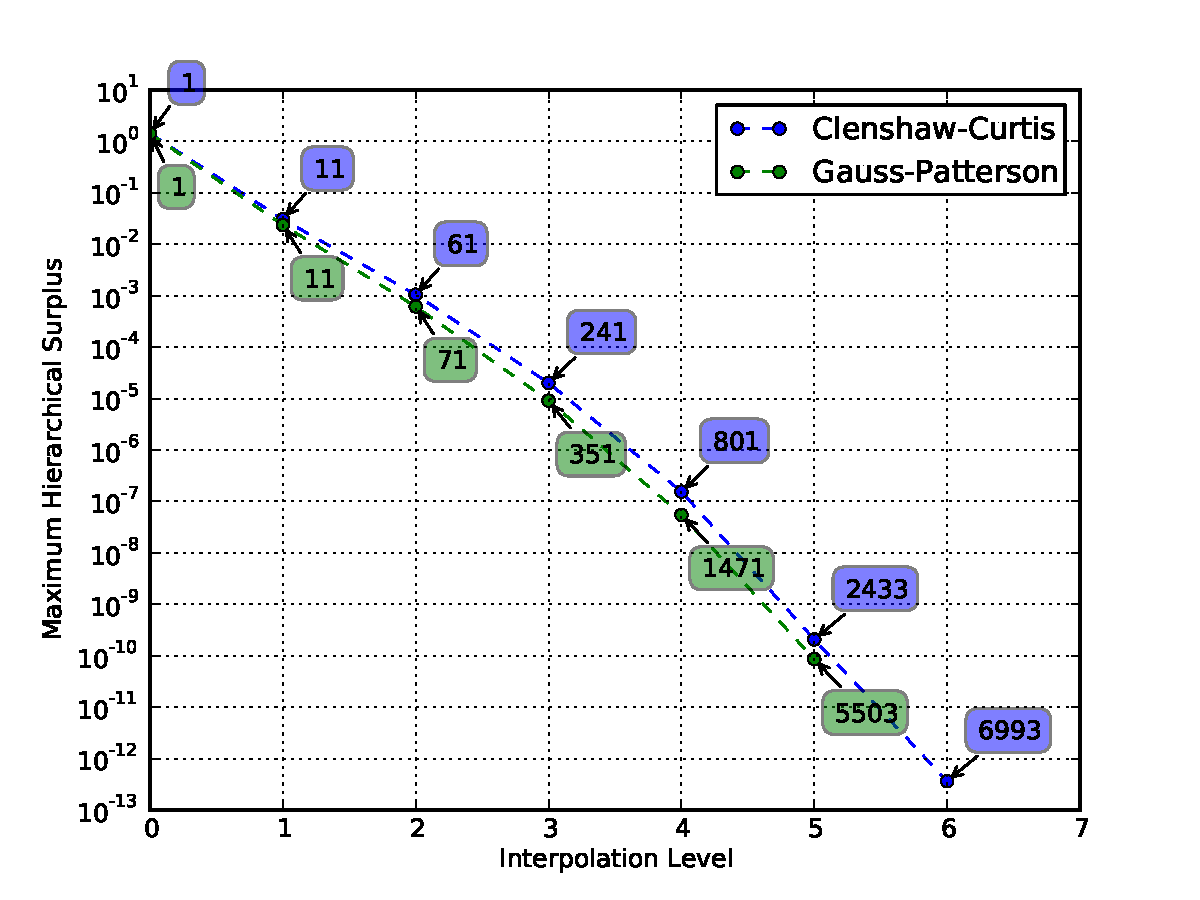
\includegraphics[scale=.75]{./Chapter3/kinf_sparse_grid_convergence.pdf}
 \end{center}
\end{figure}

From Fig. \ref{fig:kinf_sg_convergence} the Clenshaw-Curtis and Gauss-Patterson schemes perform similarly in terms of level to level convergence. However, observe that at each interpolation level the Gauss-Patterson scheme requires significantly more nodes in exchange for a small increase in convergence speed. Both schemes converge to the threshold around level five although the Gauss-Patterson scheme requires more than twice as many function evaluations to get there than Clenshaw-Curtis. Based on the graphical determination of order of convergence \cite{Boyd}, it is clear from \ref{fig:kinf_sg_convergence} that the Smolyak interpolant for $k_{\infty}$ converges geometrically.

With the Smolyak interpolation routines working as expected it's safe to apply them to an anchored-\ac{ANOVA} decomposition of $k_{\infty}$. To start, only the first order components will be built and analyzed. The first order components are relatively cheap to produce and often collectively produce very accurate reduced order models \cite{AHSGC_HighDimensions}. Afterwards, all higher order components will be added in order to show that the full anchored-\ac{ANOVA} decomposition can fully reproduce the objective function. Since $k_{\infty}$ is a function of only five random variables there is no point in adaptively constructing the reduced order model as described in Section \ref{subsec:dimension_truncation}.        

As a first comparison between all the models developed for quantifying the uncertainty in $k_{\infty}$ the mean and variance values of each model will be compared. With the exception of the variance obtained using the Sandwich Equation, each model's variance was obtained by propagating 1000 samples of Eq. $\ref{eq:sample_covariance}$ through the model. All samples produced for each model were seeded identically and so the same random numbers were drawn. The mean and variance results, along with 99\% confidence intervals, are summarized in Table \ref{table:kinf_mean_variance}. 
    
\begin{table} 
\caption[Mean and variance for TMI infinite multiplication factor.]{\label{table:kinf_mean_variance} 
Mean and variance data for the multiplication factor of an infinite TMI lattice obtained using Monte Carlo sampling. Wherever sampling was utilized the same random numbers were used.}
\centering
\small
\begin{tabular}{||c|c|c|c|c||} 
\hline \hline
\textbf{Method} & \textbf{Mean} & \textbf{99\% CI} & \textbf{Standard Dev.} & \textbf{99\% CI} \\ \hline
5D Sparse Grid CC      & 1.41562 & (1.41512, 1.41612) & 0.006168 & (0.005909, 0.006544) \\ \hline
5D Sparse Grid GP      & 1.41562 & (1.41512, 1.41612) & 0.006168 & (0.005831, 0.006544) \\ \hline
1D ANOVA CC  & 1.41560 & (1.41510, 1.41610) & 0.006168 & (0.005831, 0.006544) \\ \hline
All ANOVA CC & 1.41562 & (1.41512, 1.41612) & 0.006168 & (0.005831, 0.006544) \\ \hline
1D ANOVA GP  & 1.41560 & (1.41510, 1.41610) & 0.006168 & (0.005831, 0.006544) \\ \hline
All ANOVA GP & 1.41562 & (1.41512, 1.41612) & 0.006168 & (0.005831, 0.006544) \\ \hline
True Function & 1.41562 & (1.41512, 1.41612) & 0.006168 & (0.005831, 0.006544) \\ \hline
Sandwich               &         &                    & 0.006540 &                      \\
\hline \hline
\end{tabular}
\end{table}

The five dimensional sparse grid interpolant results are entirely self consistent with the anchored-\ac{ANOVA} results. Further, both of these methods produce identical results to those obtained using Monte Carlo sampling. Although the analytic variance from the Sandwich Equation is within the 99\% confidence bounds of each model's results, there is a notable difference due to the fact that only 1000 samples were used to obtain each model's statistics. Increasing the number of samples decreased the difference. Note that in Table \ref{table:kinf_mean_variance} the anchored-\ac{ANOVA} the reduced order models consisting of only one dimension anchored-\ac{ANOVA} components perform just as well as the full decomposition and the sparse grid interpolants over all five random variables. However, the 1D component models require only 29 function evaluations to produce, which is some ten times fewer evaluations than the 5D interpolants, and some hundred times fewer evaluations than the full decomposition. 
\begin{figure}
\caption[Cumulative knot count for constructing an anchored-\ac{ANOVA} decomposition.]{ \label{fig:kinf_numknots}
Cumulative number of knots required at each level of an anchored-\ac{ANOVA} decomposition of the multiplication factor of an infinite TMI lattice. Boxes contain the calculated standard deviation at the current level.}
 \begin{center}
  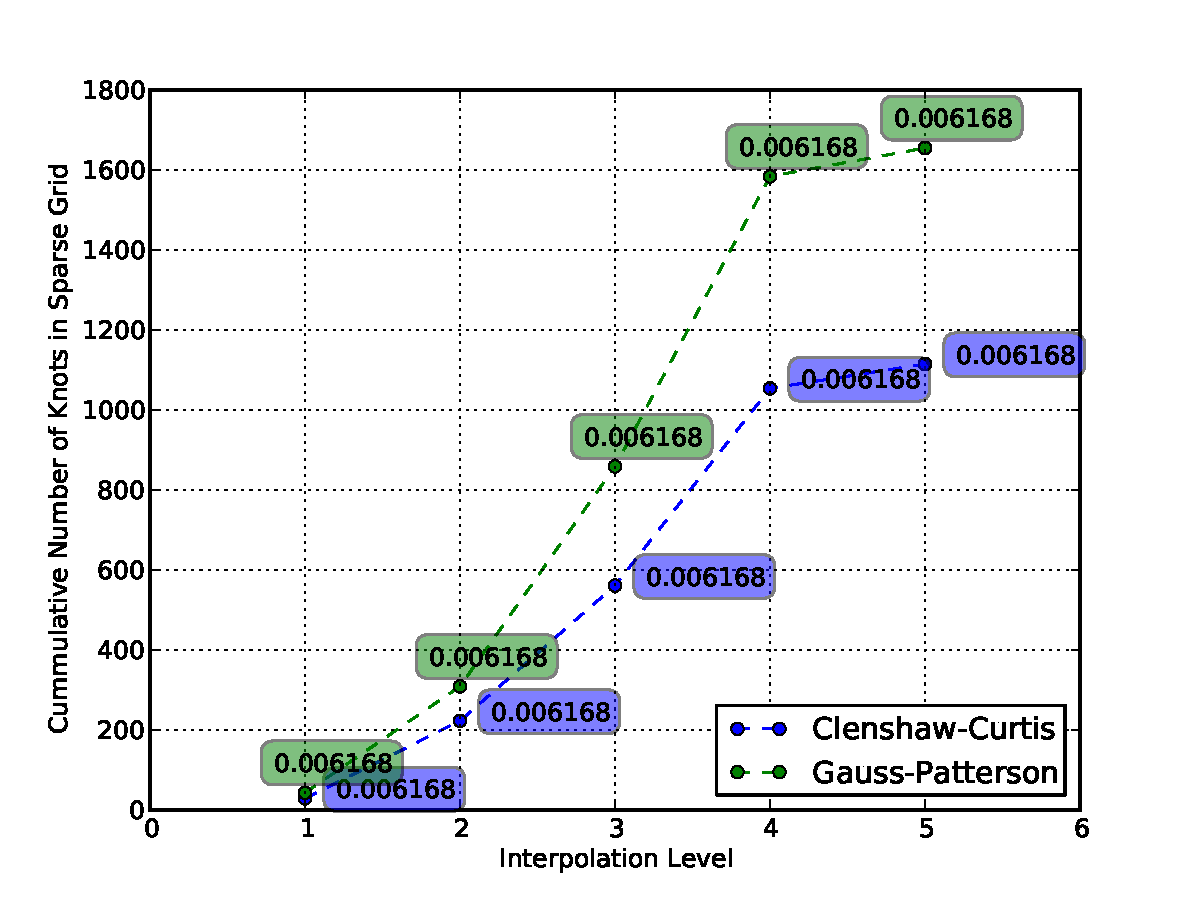
\includegraphics[scale=.75]{./Chapter3/kinf_sparse_grid_numknots.pdf}
 \end{center}
\end{figure}
The rapid convergence of the reduced order model containing only one dimensional anchored-\ac{ANOVA} components is shown in \ref{fig:kinf_numknots}. Construction of higher order components is very expensive. Fortunately for this problem, and perhaps others, construction of only one dimensional components is completely sufficient to represent the objective function. 

As another performance measure of the reduced order model methodologies, each model is used to obtain normalized sensitivity coefficients for $k_{\infty}$. Central differencing is applied to each model, with perturbations made to each cross section at a time while holding the other cross sections at their mean values. Perturbations are taken to be 1\% of each cross section's value. Using the analytic expression for $k_{\infty}$ in \ref{eq:infinite_lattice_kinf}, the central differencing results can be compared to the true sensitivity coefficients.   The results are summarized in Table \ref{table:kinf_sensitivities}. Table \ref{table:kinf_sensitivities}, sensitivity coefficients are also obtained by applying central differencing to the true function as in Eq. \ref{eq:central_diff_kinf}. 
\begin{table}
\caption{\label{table:kinf_sensitivities} 
Normalized sensitivity coefficients for the multiplication factor of an infinite TMI lattice.}
\centering
\begin{tabular}{||c|c|c|c|c|c||} 
\hline \hline
  & \multicolumn{5}{|c||}{\textbf{Normalized Sensitivity Coefficient of $k_{\infty}$}}  \\ \hline
\textbf{Method} & $\Sigma_{a_1}$ & $\Sigma_{a_2}$ & $\nu\Sigma_{f_1}$ & $\nu\Sigma_{f_2}$ & $\Sigma_{1\rightarrow 2}$ \\ \hline
5D Sparse Grid CC  & -.367551 & -.776087 & .224060 & .776010 & .143491 \\ \hline
5D Sparse Grid GP  & -.367551 & -.776087 & .224060 & .776010 & .143491 \\ \hline
1D ANOVA CC        & -.367556 & -.776098 & .224063 & .776020 & .143493 \\ \hline
All ANOVA CC       & -.367551 & -.776087 & .224060 & .776010 & .143491 \\ \hline
1D ANOVA GP        & -.367556 & -.776098 & .224063 & .776020 & .143493 \\ \hline
All ANOVA GP       & -.367551 & -.776087 & .224060 & .776010 & .143491 \\ \hline
Analytic           & -.367520 & -.775956 & .224044 & .775956 & .143476 \\ \hline
Central Difference & -.367551 & -.776089 & .224060 & .776011 & .143492 \\
\hline \hline
\end{tabular}
\end{table}
As expected, all models utilizing the central differencing formula produce self consistent sensitivity coefficients. The models differ from the analytic sensitivity coefficients only in the fourth decimal place, which is expected given the $\mathcal{O}(\Delta\Sigma^2)$ convergence  of the central differencing formula.

Finally, the performance of a Kriging surrogate, as described in section \ref{sec:kriging}, in modeling the infinite multiplication factor will be assessed. Before a Kriging surrogate is constructed the designer must agree on the number of points that will be used to construct the surrogate. As the number of points increases the accuracy of the Kriging surrogate is expected to increase. Recall that each point requires an evaluation of the true objective function, in this case Eq. \ref{eq:infinite_lattice_kinf}. Since Eq. \ref{eq:infinite_lattice_kinf} is linear relatively few sampling points are expected to exactly reproduce the objective function. Indeed, these expectations are demonstrated in
Fig. \ref{fig:kinf_kriging}.  
\begin{figure}
\caption[Reduction in Kriging surrogate error for infinite multiplication factor with increase in points.]{ \label{fig:kinf_kriging}
Reduction in Kriging surrogate error for the infinite multiplication factor as the number of points used to build the surrogate increases.}
 \begin{center}
  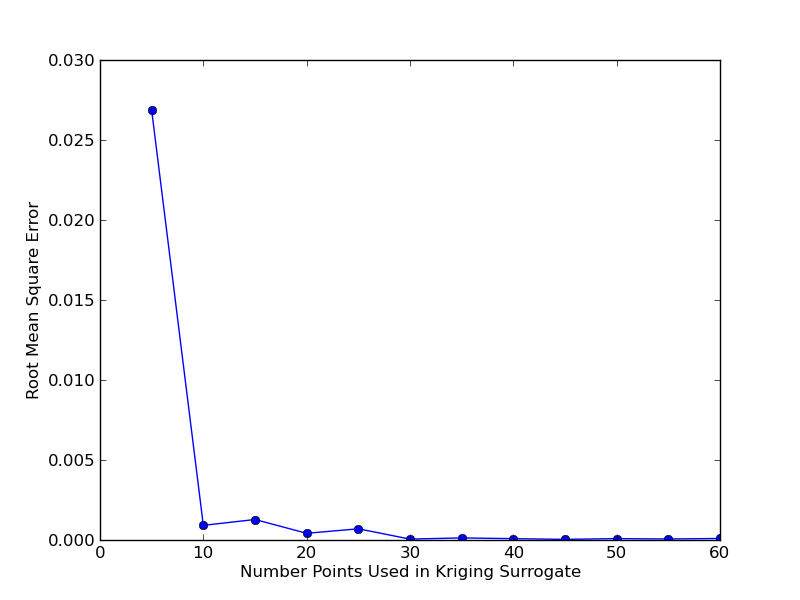
\includegraphics[scale=.75]{./Chapter3/error_vs_npoints.png}
 \end{center}
\end{figure}

In Fig. \ref{fig:kinf_kriging} the number of points used to construct the Kriging surrogate is gradually increased. For each surrogate the root mean square error is calculated by having both Eq. \ref{eq:infinite_lattice_kinf} and the surrogate evaluate the same 100 randomly chosen points in the design space. Observe that for ten evaluation points, which is twice the number of design variables in the objective function, the error essentially goes to zero. This result can be explained by Eq. \ref{eq:infinite_lattice_kinf}'s linearity and the fact that Kriging is an interpolation method, thus requiring a pair of points in each dimension for exact interpolation.     

   

% Kinetics/Thermalhydraulics 
\section{Point Kinetics/Lumped Thermal Hydraulics}
\label{sec:pointkinetics_th}

\subsection{Problem Statement}
\label{subsec:pointkinetics_th_ps}

A reduced order model based on the anchored-\ac{ANOVA} decomposition will be constructed in this section for a simple system of ordinary differential equations modeling a transient in a BN800 sodium fast cooled reactor. The physical model of the reactor consists of point kinetics to model the neutronics and lumped thermal hydraulics equations to describe temperature feedback. The coupled system is nonlinear and only has a time dependence. Previous research groups have utilized point kinetics and lumped thermal hydraulics equations to model basic reactor systems in \cite{Gilli_annals}, \cite{Gilli_mc2011}, and \cite{Housiadas}. In this section a reduced order model will be constructed for the maximum fuel temperature attained following a reactivity insertion as a function of the random variables exhibited in the description of the point kinetics/lumped thermal hydraulics system.  

The six-group point kinetics equations modeling the neutronics of a reactor consist of a balance for reactor power $P(t)$ and a balance equation for each of the six precursor concentrations $C_k(t)$. Changes in reactor power are dependent on the precursor concentration, decays constants $\lambda_k$, delayed neutron fraction $\beta$ and the mean neutron generation time $\Lambda$ as detailed in,
\begin{equation}
\label{eq:pk_power}
   \frac{dP}{dt} = \frac{\rho(T_f,T_c,t)-\beta}{\Lambda}P +
    \sum_{k=1}^6 \lambda_k C_k.
\end{equation}  
The reactivity $\rho$ depends on feedback from the fluids temperature models for the reactor fuel and coolant, which in turn depend on reactor power. The expression for each of the $k$ precursor concentrations is written as,
\begin{equation}
\label{eq:pk_precursors}
   \frac{dC_k}{dt} = -\lambda_k C_k +
    \frac{\beta_k}{\Lambda}P.
\end{equation}
As for the ordinary differential equations describing the behavior of the reactor coolant system, two coupled equations suffice. For the fuel temperature $T_f$, the following lumped model is used,
\begin{equation}
\label{eq:pk_fuel}
   M_f c_{pf}\frac{dT_f}{dt} = P + Ah(T_c-T_f)
\end{equation}
where $M_f$ is the lump fuel mass, $c_{pf}$ is the specific heat capacity of the fuel, $A$ is the heat transfer surface, and $h$ is the heat transfer coefficient between the coolant and reactor fuel. Finally, the coolant temperature is described as,
\begin{equation}
\label{eq:pk_coolant}
   M_c c_{pc}\left(\frac{dT_c}{dt} +v \frac{T_c - T_{in}}{L}\right) = 
    Ah(T_f-T_c)
\end{equation}
where $M_c$ is the lump coolant mass, $c_{pc}$ is the specific heat capacity of the coolant, $L$ is the coolant channel length, $v$ is the coolant flow velocity, and $T_{in}$ is the inlet coolant temperature. The initial conditions for $P$, $C_k$, $T_f$, and $T_c$ depend on the initial power in the reactor $P_0$ before any kind of transient occurs and are listed in \ref{eq:pk_initial_conds}. 
\begin{eqnarray}
\label{eq:pk_initial_conds}
   P(0) &=& P_0 \\ 
   C_k(0) &=& \frac{\beta_k}{\lambda_k\Lambda}P_0 \nonumber \\
   T_f(0) &=& T_c(0) + \frac{P_0}{Ah} \nonumber \\
   T_c(0) &=& T_{in} + \frac{P_0L}{M_c c_{pc}v} \nonumber
\end{eqnarray}
Serving as the coupling device between the lumped thermal hydraulics model and point kinetics model is the reactivity, which is proportional to the coolant temperature and the fuel temperature. Of course, any external reactivity $\rho_{ex}$ added to the reactor is also a contributor. The time dependent reactivity is given explicitly as,
\begin{equation}
\label{eq:pk_reactivity}
   \rho(T_f,T_c,t) = \rho_{ex} + \alpha_d(T_f - T_f(0))
    + \alpha_c(T_c - T_c(0))
\end{equation}
where $\alpha_d$ and $\alpha_c$ are the doppler and coolant coefficients of reactivity, respectively.  

The equations in \ref{eq:pk_power}, \ref{eq:pk_precursors}, \ref{eq:pk_coolant}, and \ref{eq:pk_fuel} are used to model the transient resulting from a half sawtooth external reactivity insertion, as shown in \ref{eq:pk_half_sawtooth}. 
\begin{equation}
\label{eq:pk_half_sawtooth}
   \rho_{ex}(t) = \left\{
    \begin{array}{cr}
     t\rho_{max}/20 & t \leq 20 \\
     0                      & t > 20 
    \end{array}
    \right.
\end{equation}
By treating the coefficients in the point kinetics/lumped thermal hydraulics model as random variables, the objective function investigates the response surface for the maximum fuel temperature attained during transient. The reduced order methodologies will be tested against the stated problem. A depiction of the transient at the random variables' mean values, along with the external reactivity is shown in Figure \ref{fig:pk_transient}.  
\begin{figure}
\caption[Half sawtooth external reactivity insertion transient behavior.]{ \label{fig:pk_transient}
Transient resulting from a half sawtooth external reactivity insertion, as modeled using the mean parameter values of the point kinetics/lumped thermal hydraulics system.}
 \begin{center}
  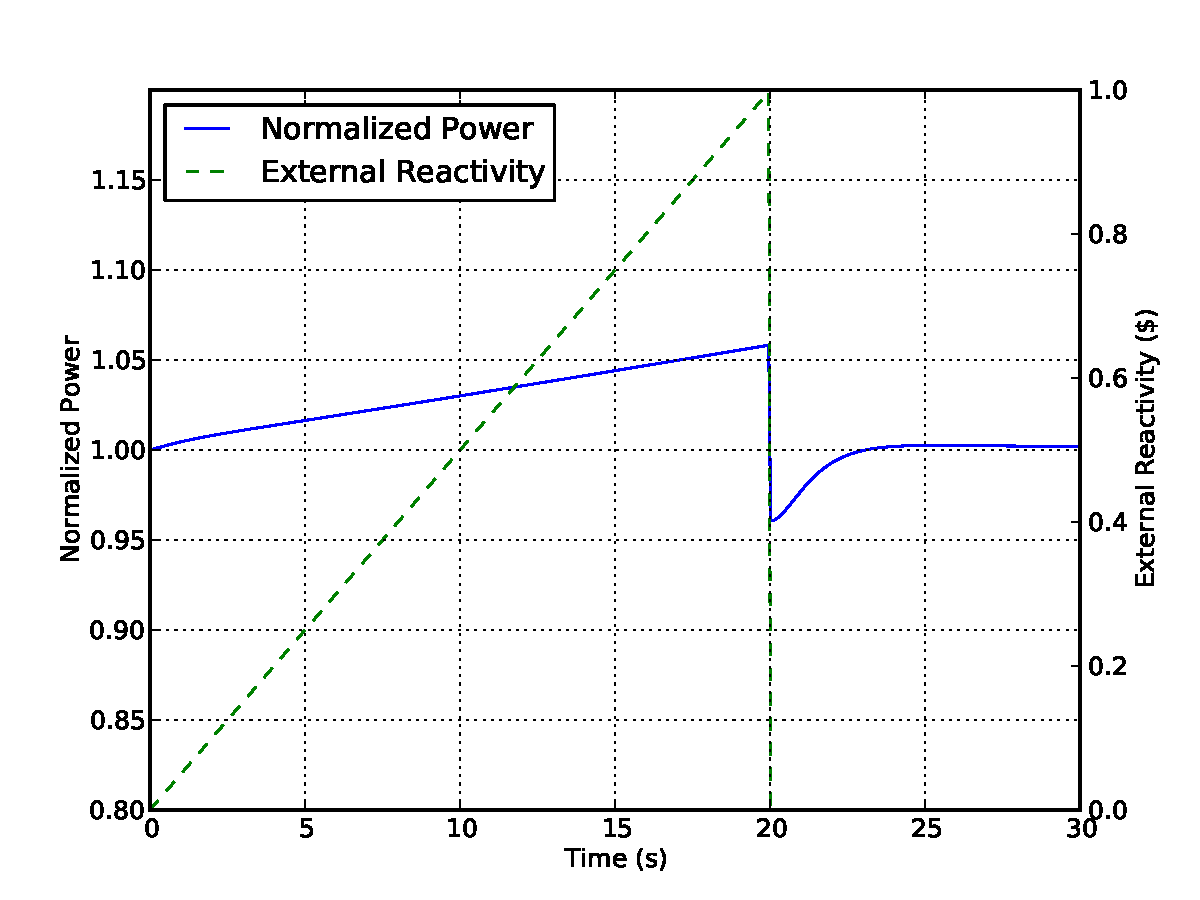
\includegraphics[scale=.75]{./Chapter3/pk_power.pdf}
 \end{center}
\end{figure}
A total of twenty two random variables will be investigated for their affect on the maximum fuel temperature attained during transient. The random variables' mean values, along with their standard deviations are listed in \ref{table:pkinetics_parameters}. Note that all standard deviations are taken to be 5\% of the mean value. All random variables are assumed to be independent of one another, as was assumed in \cite{Gilli_mc2011}. 
\begin{table} 
\caption[Parameter values used in a point kinetics/lumped thermal hydraulics model of a BN800 fast sodium cooled reactor.]{\label{table:pkinetics_parameters} 
Mean parameter values used in the point kinetics/lumped thermal hydraulics model for the analysis of a BN800 fast sodium cooled reactor.}
\centering
\begin{tabular}{||c|c|c|c||} 
\hline \hline
\textbf{Random Variable} & \textbf{Units} & \textbf{Mean} & \textbf{Standard Dev.} \\ \hline
$\lambda_1$  &  $s^{-1}$      &  1.24E-02  &  6.20e-04  \\ \hline
$\lambda_2$  &  $s^{-1}$      &  3.05E-02  &  1.52e-03  \\ \hline
$\lambda_3$  &  $s^{-1}$      &  1.11E-01  &  5.55e-03  \\ \hline
$\lambda_4$  &  $s^{-1}$      &  3.01E-01  &  1.50e-02  \\ \hline
$\lambda_5$  &  $s^{-1}$      &  1.14E+00  &  5.70e-02  \\ \hline
$\lambda_6$  &  $s^{-1}$      &  3.01E+00  &  1.50e-01  \\ \hline
$\beta_1$    &                &  9.00E-05  &  4.50e-06  \\ \hline
$\beta_2$    &                &  8.53E-04  &  4.26e-05  \\ \hline
$\beta_3$    &                &  7.00E-04  &  3.50e-05  \\ \hline
$\beta_4$    &                &  1.40E-03  &  7.00e-05  \\ \hline
$\beta_5$    &                &  6.00E-04  &  3.00e-05  \\ \hline
$\beta_6$    &                &  5.50E-04  &  2.75e-05  \\ \hline
$\Lambda$    &  $s$           &  4.00E-07  &  2.00e-08  \\ \hline
$Ah$         &  $kW/K$        &  2.50E+06  &  1.25e+05  \\ \hline
$M_c$        &  $kg$          &  1.16E+03  &  5.84e+01  \\ \hline
$M_f$        &  $kg$          &  9.67E+03  &  4.83e+02  \\ \hline
$c_{pc}$     &  $J/kg\cdot K$ &  1.20E+03  &  6.00e+01  \\ \hline
$c_{pf}$     &  $J/kg\cdot K$ &  5.00E+02  &  2.50e+01  \\ \hline
$v$          &  $m/s$         &  7.50E+00  &  3.75e-01  \\ \hline
$\alpha_d $  &  $pcm/K$       &  6.87E-06  &  3.43e-07  \\ \hline
$\alpha_c$   &  $pcm/K$       &  1.23E-06  &  6.15e-08  \\ \hline
$\rho_{max}$ &                &  4.19E-04  &  2.09e-05  \\ 
\hline \hline
\end{tabular}
\end{table}
A plot of the fuel temperature as a function of time due to the external reactivity profile shown in the same figure is depicted in Figure \ref{fig:pk_fuel_temp}. 
\begin{figure}[!htb]
\caption[Fuel temperature transient resulting from a half sawtooth reactivity insertion.]{ \label{fig:pk_fuel_temp}
Fuel temperature transient resulting from a half sawtooth reactivity insertion. All parameters in the coupled point kinetics/lumped thermal hydraulics equations are held at their mean values. 
}
 \begin{center}
  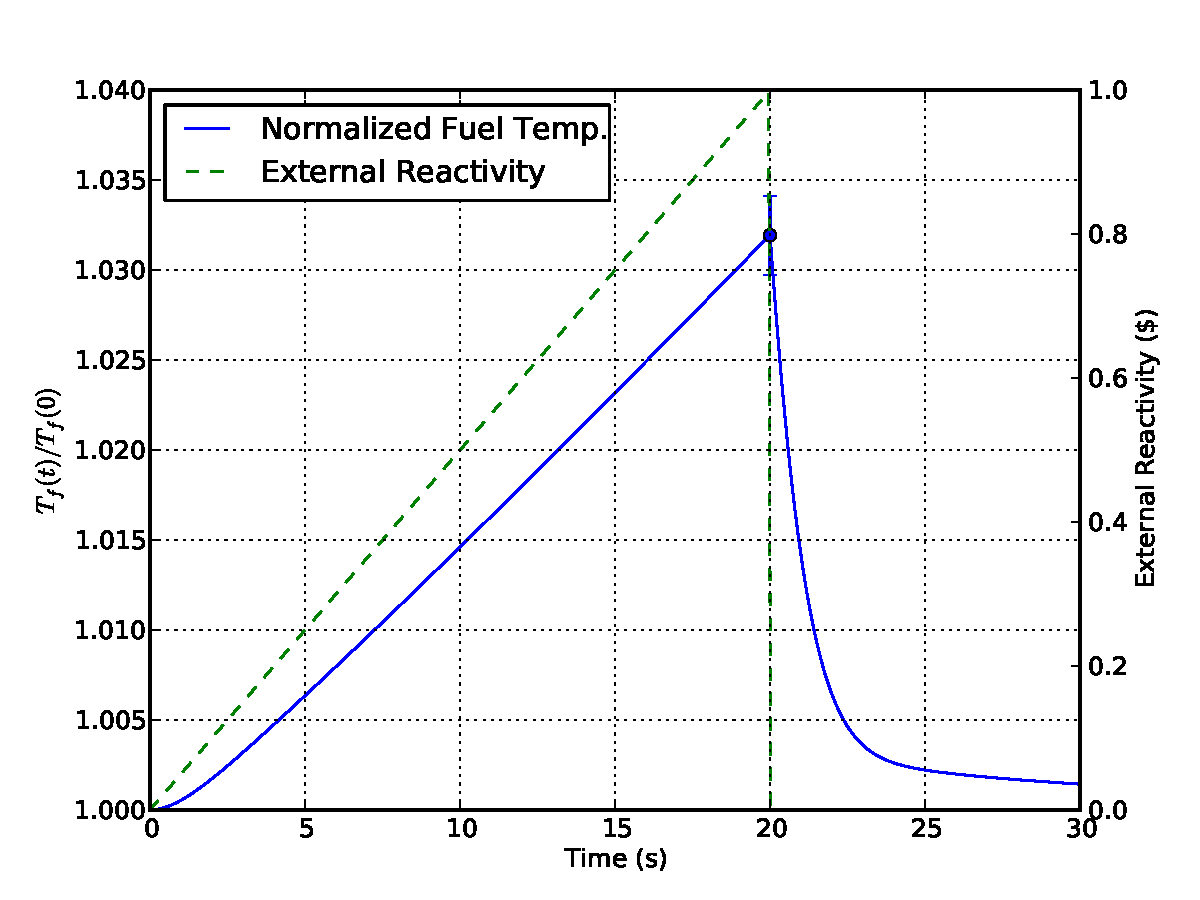
\includegraphics[scale=.75]{./Chapter3/pk_fueltemp.pdf}
 \end{center}
\end{figure}

\subsection{Analysis}
\label{subsec:pointkinetics_th_analysis}

An adaptive reduced order model, whose formulation is summarized in Algorithm \ref{code:rom_algorithm}, will be created for the problem described in section \ref{subsec:pointkinetics_th_ps}. The reduced order model will be investigated for its ability to reproduce statistics of interest by comparing its results with those obtained from sampling the true function. As described in Algorithm \ref{code:rom_algorithm}, the first step in creating a reduced order model for the maximum fuel temperature is to construct all first order components in the anchored-\ac{ANOVA} decomposition and to identify the important ones. The sparse grids comprising the reduced order model are assumed to be converged when the maximum hierarchical surplus for a given level is less than $10^{-5}$. Consequently, at least five digits of accuracy are expected. Important dimensions are those whose normalized sensitivity index in Eq. \ref{eq:anova_sensitivity} exceeds 5\%.

From Figure \ref{fig:pk_importance_pie} the "important" variables are identified to be $Ah$, $\alpha_d$, and $\rho_{max}$. Collectively these three "important" random variables comprise 82\% of the total sensitivity. 
\begin{figure}[!htb]
\caption[Normalized sensitivity indices for random variables comprising the coupled point kinetics/lumped thermal hydraulics equations.]{ \label{fig:pk_importance_pie}
Normalized sensitivity indices for all random variables comprising the coupled point kinetics/lumped thermal hydraulics equations. The effects of all $\beta_k$ and $\lambda_k$ have been lumped into single $\beta$ and $\lambda$ effects, respectively. 
}
 \begin{center}
  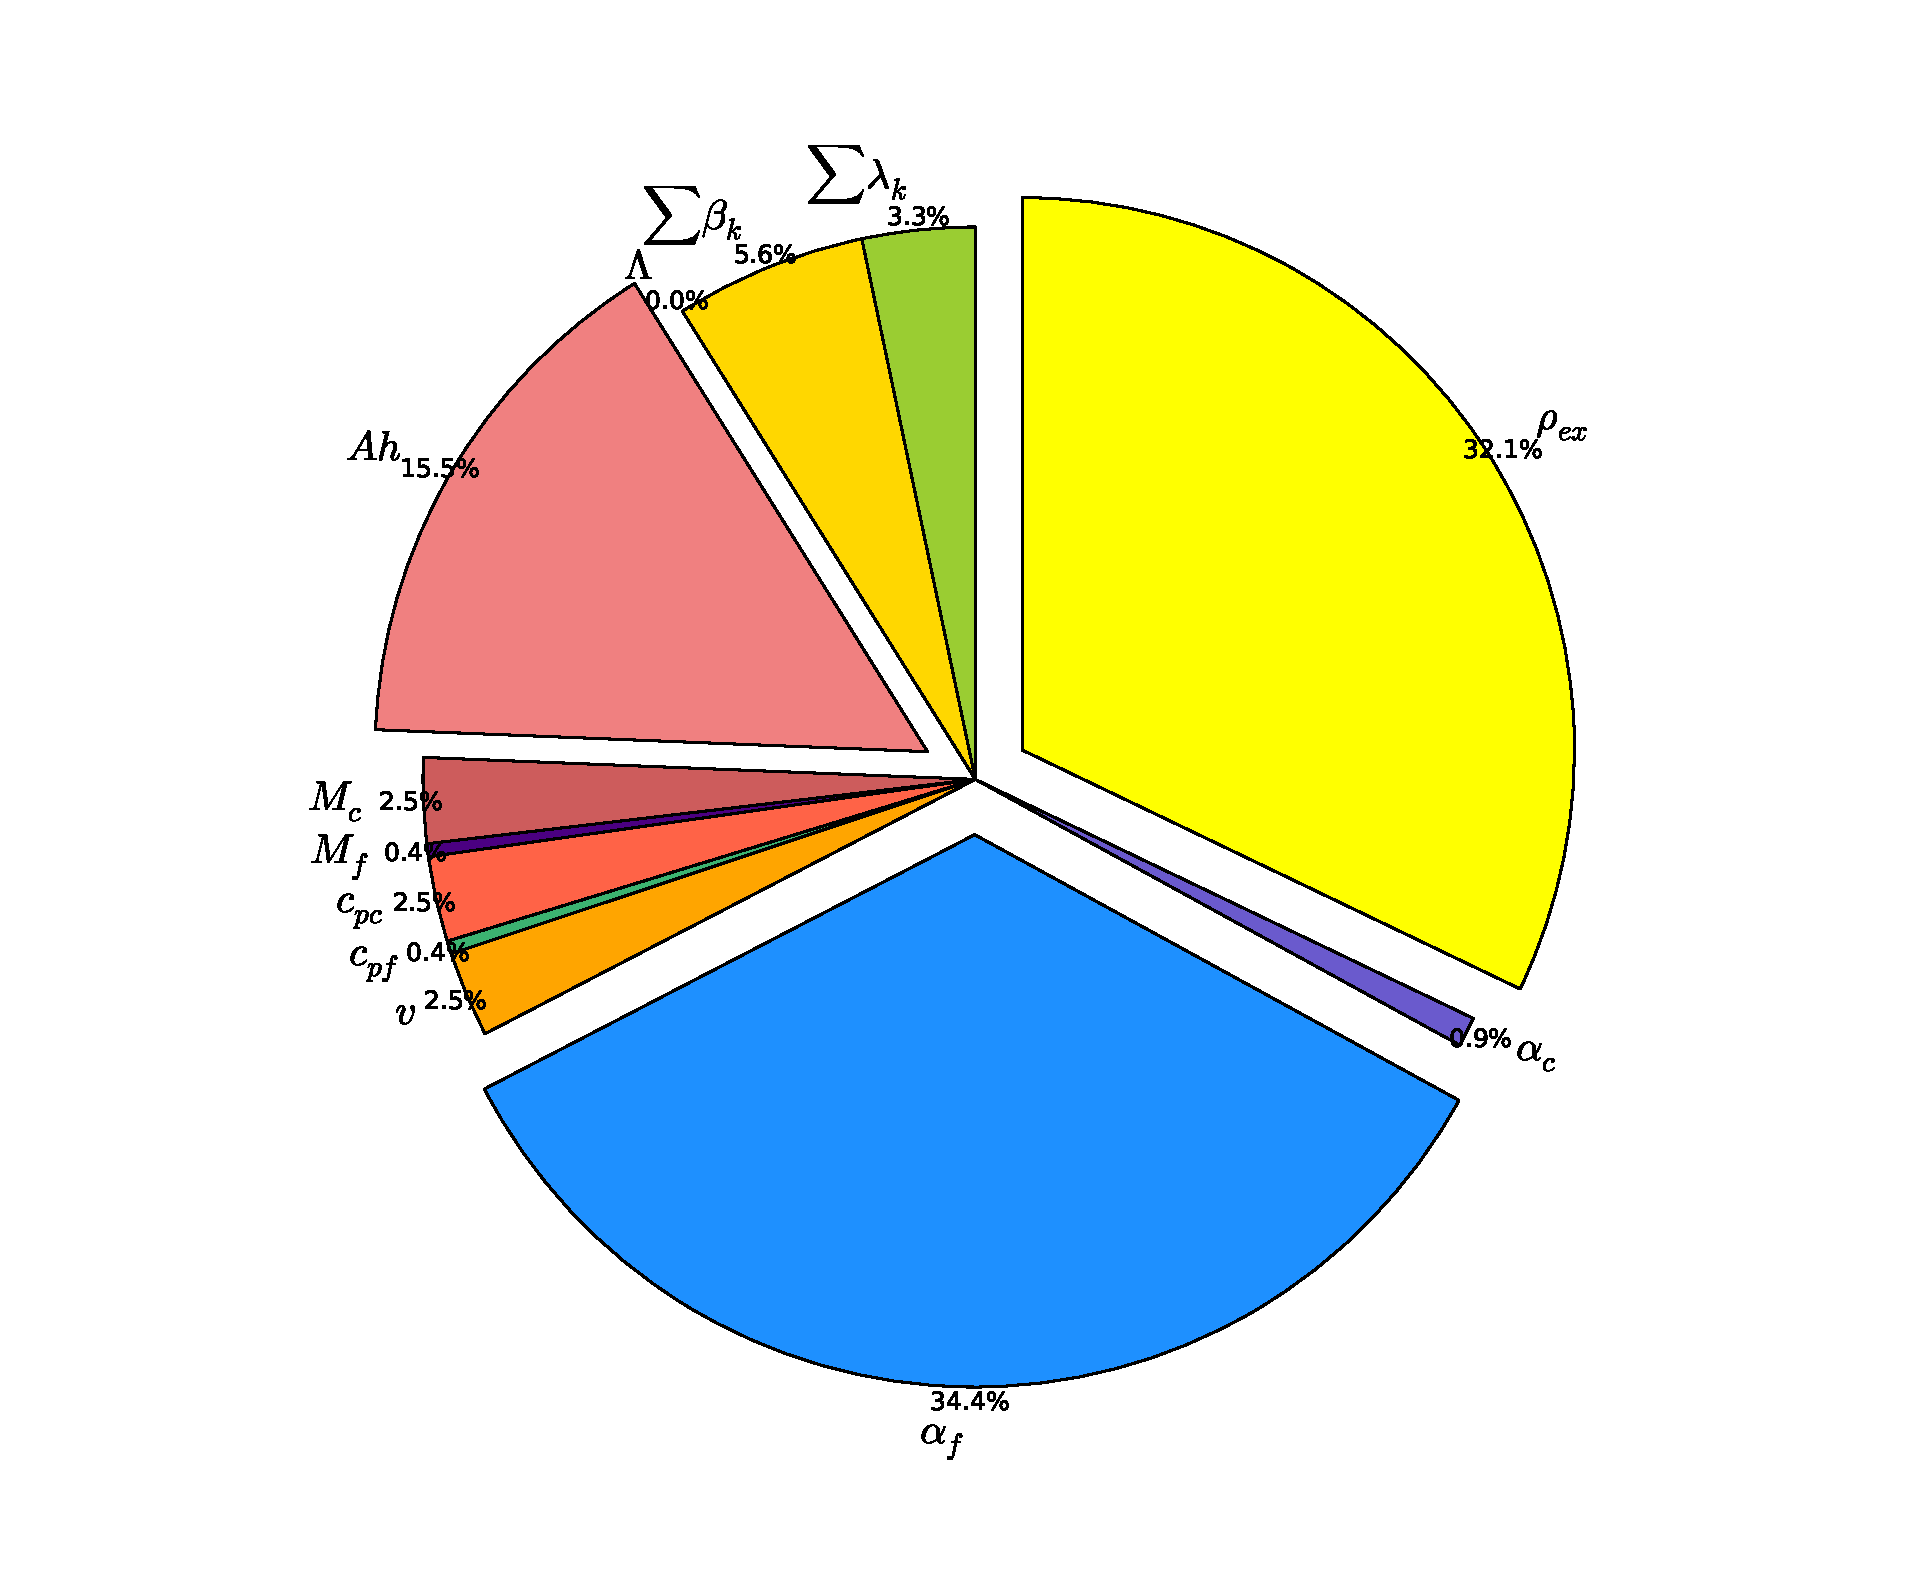
\includegraphics[scale=.5]{./Chapter3/pk_importance_pie.pdf}
 \end{center}
\end{figure}
The indication that the maximum fuel temperature is sensitive to the heat transfer $Ah$ from fuel to coolant is not surprising since in Eq. \ref{eq:pk_fuel} the fuel temperature is directly proportional to $Ah$. Further, the random variables $\rho_{max}$ and $\alpha_d$ determine the slope of the increase in fuel temperature, as seen in Figure \ref{fig:pk_fuel_temp}, and so a strong sensitivity to these random variables is expected. The sensitivity of the maximum fuel temperature to $\alpha_c$ is not as great since the increase in coolant temperature during the transient is significantly smaller than the rise in fuel temperature. Relatively weak sensitivity to $M_f$ and $c_{pf}$ can perhaps be attributed to cancellation of error since these two variables are multiplied together.

With only three random variables deemed as "important" only three second order anchored-\ac{ANOVA} components must be built for the reduced order model. Neglecting any convergence criteria, third order component describing the interaction effects among the three important random variables is also built. A summary of the total number of function evaluations needed to construct the adaptive reduced order model for the maximum fuel temperature is shown in Figure \ref{fig:pk_sparse_grid_numknots}.          
\begin{figure}[!htb]
\caption[Cumulative number of knots for constructing a reduced order model of the maximum fuel temperature in the point kinetics/lumped thermal hydraulics model.]{\label{fig:pk_sparse_grid_numknots}
Number of knots needed to adaptively construct a reduced order model for the maximum fuel temperature in both the Clenshaw-Curtis and Gauss-Patterson schemes. Boxed values state the standard deviation calculated at each level.  
}
 \begin{center}
  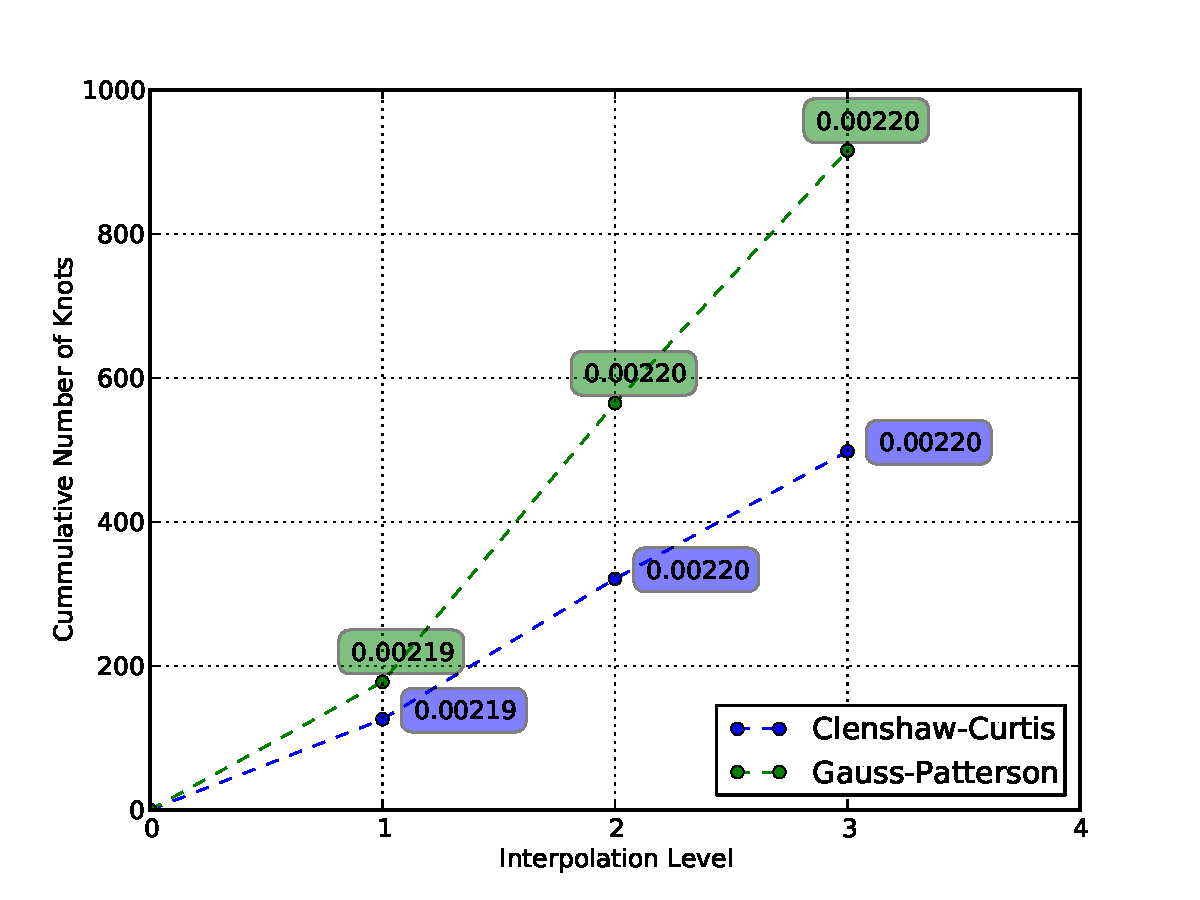
\includegraphics[scale=.75]{./Chapter3/pk_sparse_grid_numknots.pdf}
 \end{center}
\end{figure}
The Gauss-Patterson scheme required almost twice as many knots as Clenshaw-Curtis to adaptively build the reduced order model. From Figure \ref{fig:pk_sparse_grid_numknots} it's clear that the reduced order model consisting of only one dimensional components is effectively just as accurate as the full model, but requiring only 126 function evaluations to build using Clenshaw-Curtis. To see how well the reduced order models are able to reproduce the mean and variance of the true function Monte Carlo simulation is utilized. The models produced using anchored-\ac{ANOVA} decomposition with superposition dimensions of one and three are sampled along with the true function. Mean, variance, and pertinent 99\% confidence intervals for the sampling are summarized in Table \ref{table:pk_mean_variance}. A total of 1000 samples were used for each method, each using the same random numbers.      
\begin{table}[!htb] 
\caption[Mean and variance data for maximum fuel temperature achieved during transient.]{\label{table:pk_mean_variance} 
Mean and variance data for the maximum fuel temperature achieved during transient obtained using Monte Carlo sampling. The same random numbers were used for all 1000 samples for each method.}
\centering
\small
\begin{tabular}{||c|c|c|c|c||} 
\hline \hline
\textbf{Method} & \textbf{Mean} & \textbf{99\% CI} & \textbf{Standard Dev.} & \textbf{99\% CI} \\ \hline
1D ANOVA CC  & 1.03193 & (1.03175, 1.03211) & 0.002187 & (0.002068, 0.002320) \\ \hline
All ANOVA CC & 1.03193 & (1.03175, 1.03211) & 0.002196 & (0.002076, 0.002330) \\ \hline
1D ANOVA GP  & 1.03193 & (1.03175, 1.03211) & 0.002187 & (0.002068, 0.002320) \\ \hline
All ANOVA GP & 1.03193 & (1.03175, 1.03211) & 0.002196 & (0.002076, 0.002330) \\ \hline
True Function & 1.03193 & (1.03175, 1.03211) & 0.002196 & (0.002076, 0.002330) \\ 
\hline \hline
\end{tabular}
\end{table}
As evidenced in Table \ref{table:pk_mean_variance} the statistical results for each method are consistent. While the reduced order model with superposition dimension of three is able to replicate the Monte Carlo results to five significant figures, the expected accuracy, the order-one superposition model is slightly short. Of course, this is due to the absence of higher order components. However, the proximity of the order-one superposition model's results to the true results indicate that for this problem the higher order components do not have a significant impact. To further verify the ability of the reduced order models to accurately reproduce basic statistical moments, the probability distributions for the normalized maximum fuel temperature produced by each model are compared in Figure \ref{fig:pk_histograms}. 
\begin{figure}[!htb]
\caption{\label{fig:pk_histograms}
Histograms produced by sampling the true function, order-one superposition reduced order model, and the full adaptive reduced order model.  
}
 \begin{center}
  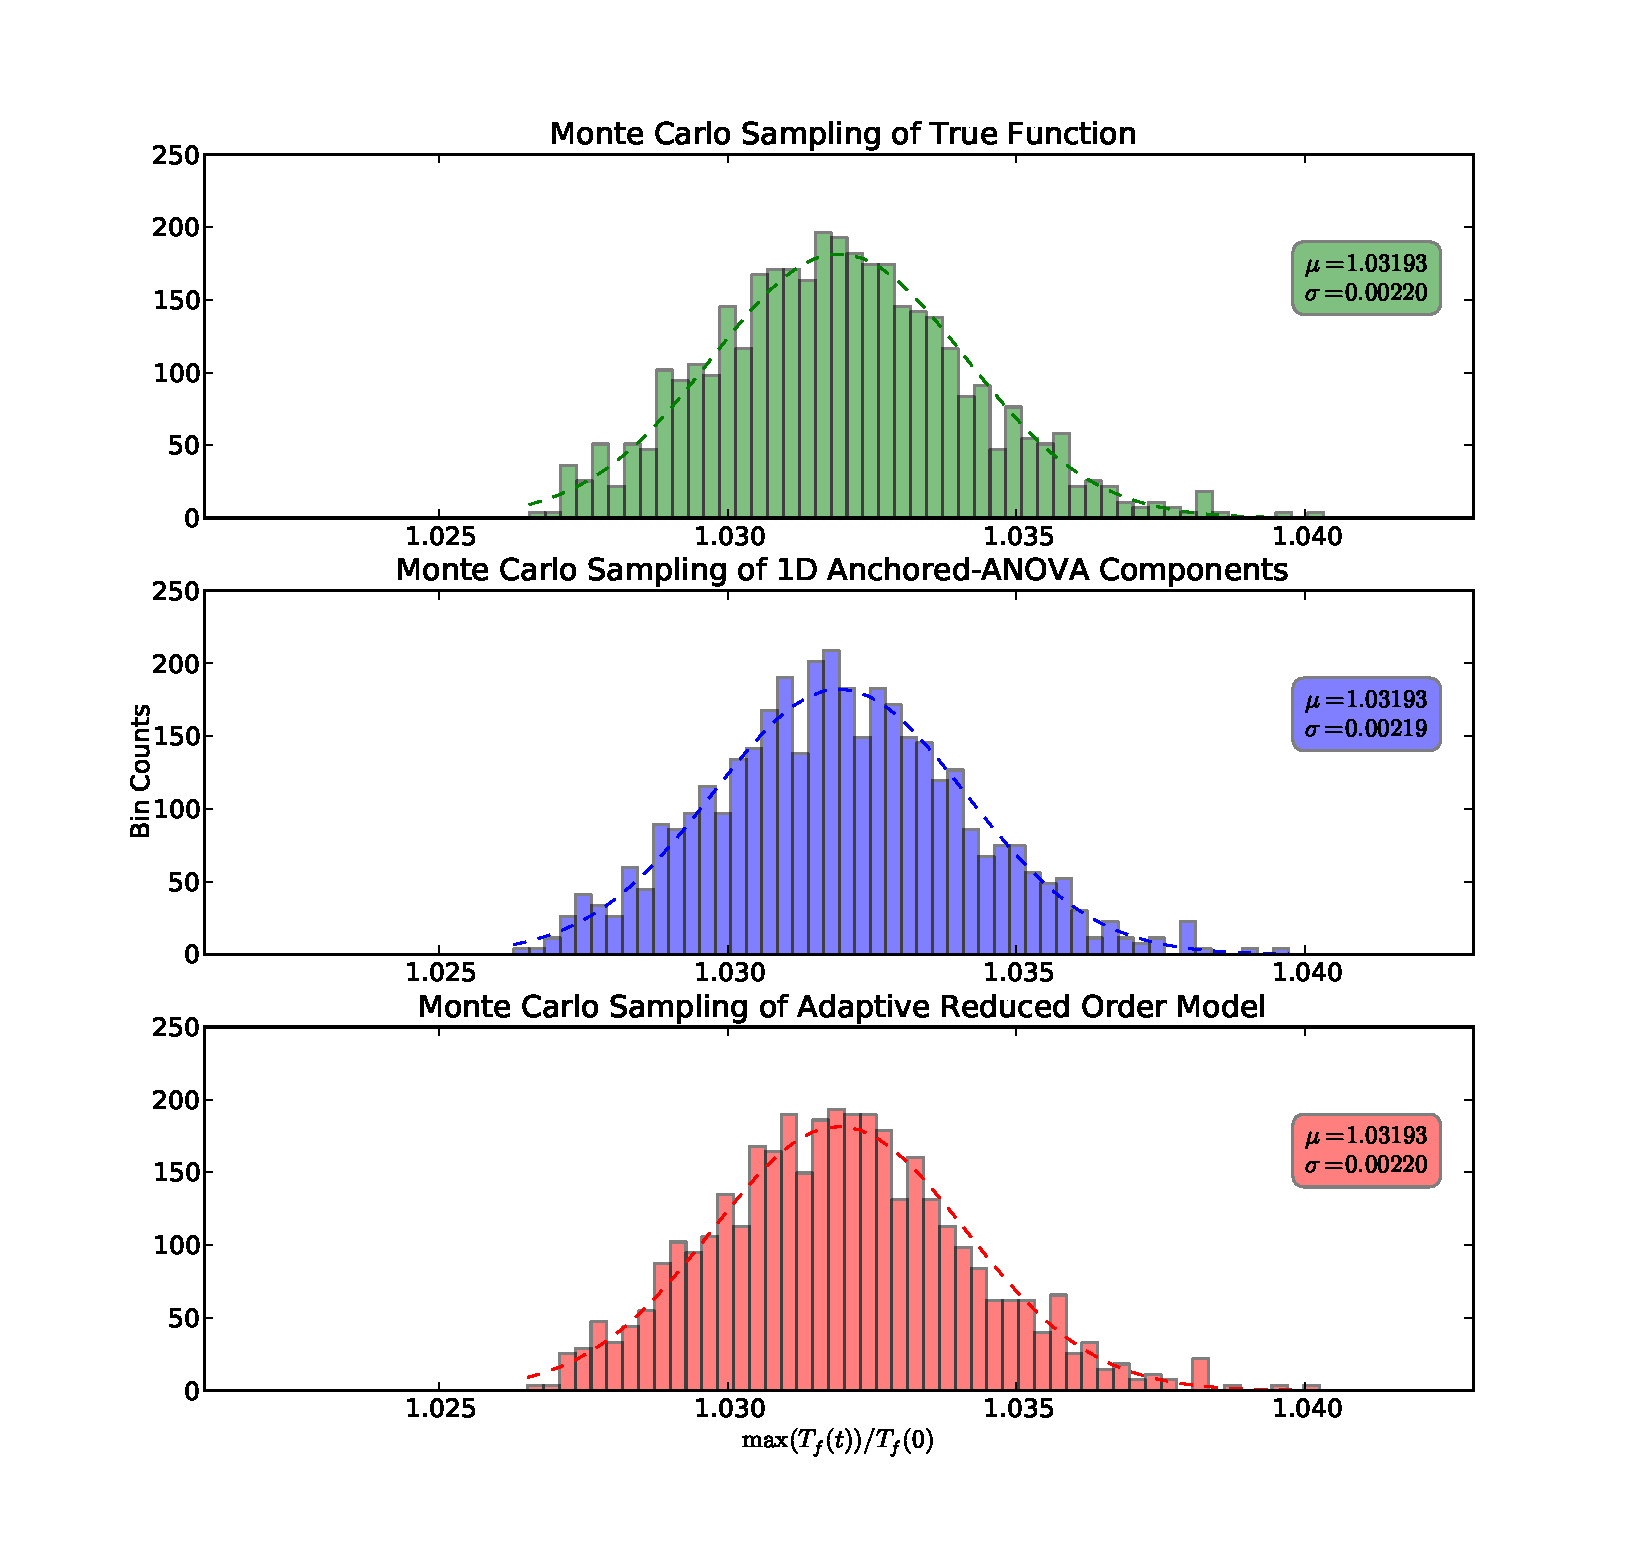
\includegraphics[scale=.58]{./Chapter3/pk_histograms.pdf}
 \end{center}
\end{figure}
All of the tested reduced order models are able to reproduce the Gaussian probability distribution for the normalized maximum fuel temperature. 

As done in section \ref{subsec:kinf_analysis}, a sensitivity analysis will be completed for the reduced order model and compared to the normalized sensitivity coefficients obtained using central differencing. From Table \ref{table:pk_sensitivities} notice that the largest sensitivity coefficients are those of the random variables deemed "important" using the adaptive reduced order model algorithm. Only the sensitivity coefficients for the Clenshaw-Curtis sparse grid are shown in Table \ref{table:pk_sensitivities} since the Gauss-Patterson sparse grid returns identical results. The normalized sensitivity coefficients calculated using the reduced order models are the same as those calculated using central differencing to the expected number of significant digits.   
\begin{table}[!htb] 
\caption{\label{table:pk_sensitivities} 
Normalized sensitivity coefficients of the maximum fuel temperature to random variables.}
\centering
\begin{tabular}{||c|c|c|c||} 
\hline \hline
\textbf{Random Variable} & \textbf{1D ANOVA CC} & \textbf{All ANOVA CC} & \textbf{Central Diff.} \\ \hline
$\lambda_1$  &  3.7894E-05 &  3.7894E-05 &  3.7895E-05 \\ \hline
$\lambda_2$  &  7.0387E-04 &  7.0387E-04 &  7.0387E-04 \\ \hline
$\lambda_3$  &  8.4244E-04 &  8.4244E-04 &  8.4215E-04 \\ \hline
$\lambda_4$  &  9.7308E-04 &  9.7309E-04 &  9.7379E-04 \\ \hline
$\lambda_5$  &  1.1572E-04 &  1.1572E-04 &  1.1607E-04 \\ \hline
$\lambda_6$  &  4.4638E-05 &  4.4639E-05 &  4.0498E-05 \\ \hline
$\beta_1$    & -3.2992E-04 & -3.2992E-04 & -3.2976E-04 \\ \hline
$\beta_2$    & -2.6582E-03 & -2.6582E-03 & -2.6616E-03 \\ \hline
$\beta_3$    & -1.1953E-03 & -1.1953E-03 & -1.2040E-03 \\ \hline
$\beta_4$    & -1.0129E-03 & -1.0129E-03 & -1.0232E-03 \\ \hline
$\beta_5$    & -1.1689E-04 & -1.1689E-04 & -1.1810E-04 \\ \hline
$\beta_6$    & -4.0718E-05 & -4.0718E-05 & -4.1134E-05 \\ \hline
$\Lambda$    & -8.9294E-08 & -8.9295E-08 & -8.9364E-08 \\ \hline
$Ah$         &  1.2553E-02 &  1.2553E-02 &  1.2584E-02 \\ \hline
$M_c$        &  1.8753E-03 &  1.8753E-03 &  1.8716E-03 \\ \hline
$M_f$        & -3.6695E-04 & -3.6695E-04 & -3.6360E-04 \\ \hline
$c_{pc}$     &  1.8753E-03 &  1.8753E-03 &  1.8903E-03 \\ \hline
$c_{pf}$     & -3.6695E-04 & -3.6695E-04 & -3.5976E-04 \\ \hline
$v$          &  1.8838E-03 &  1.8839E-03 &  1.9177E-03 \\ \hline
$\alpha_d $  & -2.6655E-02 & -2.6656E-02 & -2.6625E-02 \\ \hline
$\alpha_c$   &  8.4387E-04 &  8.4387E-04 &  8.7194E-04 \\ \hline
$\rho_{max}$ &  3.1164E-02 &  3.1164E-02 &  3.1272E-02 \\ 
\hline \hline
\end{tabular}
\end{table}

To further analyze the coupled point kinetics/lumped thermal hydraulics problem in hand, Morris' algorithm is applied, as described in section \ref{subsec:morris_algorithm}. As previously described, algorithm \ref{code:morris_algorithm} aims to identify the design variables that have the greatest influence on an objective function's behavior, which in this case is the fuel temperature. To effectively determine such design variables it is convenient to plot the mean against the standard deviation of each design variable's elementary effects. From the problem at hand, the elementary effect statistics are plotted in Fig. \ref{fig:kth_important_vars}.     
\begin{figure}[!htb]
\caption{\label{fig:kth_important_vars}
Statistics of each design variable's elementary effects, as applied to the coupled point kinetics/lumped thermal hydraulics problem.   
}
 \begin{center}
  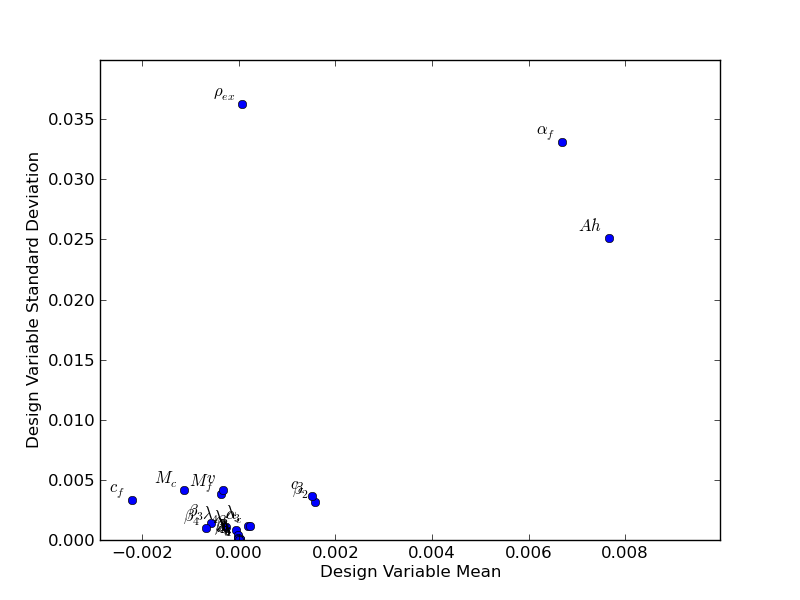
\includegraphics[scale=.75]{./Chapter3/importantvariables.png}
 \end{center}
\end{figure}
Figure \ref{fig:kth_important_vars} was obtained using five divisions and ten elementary effects per design variable. Observe how eighteen of the twenty two points are clustered around the origin, implying that each of these clustered variables have minimal influence on the fuel temperature. In contrast, the variables $\rho_{ex}$, $\alpha_f$, and $Ah$ are likely to be primary contributors. The results of Fig. \ref{fig:kth_important_vars} are entirely consistent with Fig. \ref{fig:pk_importance_pie}, which also identifies the variables $\rho_{ex}$, $\alpha_f$, and $Ah$ as being principally important.      

Now, with the three key variables identified a Kriging surrogate is constructed for the normalized fuel temperature. Sampling the three-dimensional surrogate 1000 times, as done to obtain the results in Table \ref{table:pk_mean_variance}, a mean normalized temperature of $1.03198 \pm 0.002299$ was obtained which is well within the $99\%$ confidence interval of the sampled true result. Note that some of the statistical discrepancies being observed can be attributed to the fact that the same random number were not used in the evaluation of the surrogate and true function. 


% TMI Minicore
\section{\ac{TMI} Minicore}
\label{sec:tmi_minicore}

\subsection{Problem Statement}
\label{subsec:tmi_minicore_ps}

The previous two problems dealt with relatively simple functions that don't require industrial engineering codes to solve. However, the main intention of this thesis is to construct reduced order models for computer codes that aim to model large and complex engineering systems. Interaction with such computer codes consist of input and output files; the governing equations and their solvers are rarely seen. The primary purpose of this demonstration problem is to show that the same algorithms applied to analyze the previous problems are also functional when applied to engineering computer codes.

In this demonstration problem the reactor core simulator code \ac{PARCS} \cite{PARCS} is applied to the \ac{TMI} minicore described in the first phase of the \ac{UAM} Benchmark \cite{UAM_Benchmark}. The minicore problem consists of a three-by-three fuel assembly configuration with reflector blocks placed around the assemblies, as seen in Figure \ref{fig:tmi_minicore}. In the minicore the central assembly is rodded while the periphery fuel assemblies are unrodded. Vacuum boundary conditions are applied. The few-group, homogenized cross section description for each fuel assembly consists of transport, absorption, nu-fission, and scatter cross sections along with values for \ac{ADFs}. For a two-group problem the total number of cross sections to describe an assembly is nine. Since the homogenized reflector region does not support fission only seven homogenized cross sections are required to describe it. Consequently, to model the minicore configuration in Fig. \ref{fig:tmi_minicore} in \ac{PARCS} a total of twenty five homogenzied, two-group cross sections are needed.  
\begin{figure}[!htb]
\caption{\label{fig:tmi_minicore}
\ac{TMI} minicore configuration used for analysis, as defined in the \ac{UAM} Benchmark specifications.}
 \begin{center}
  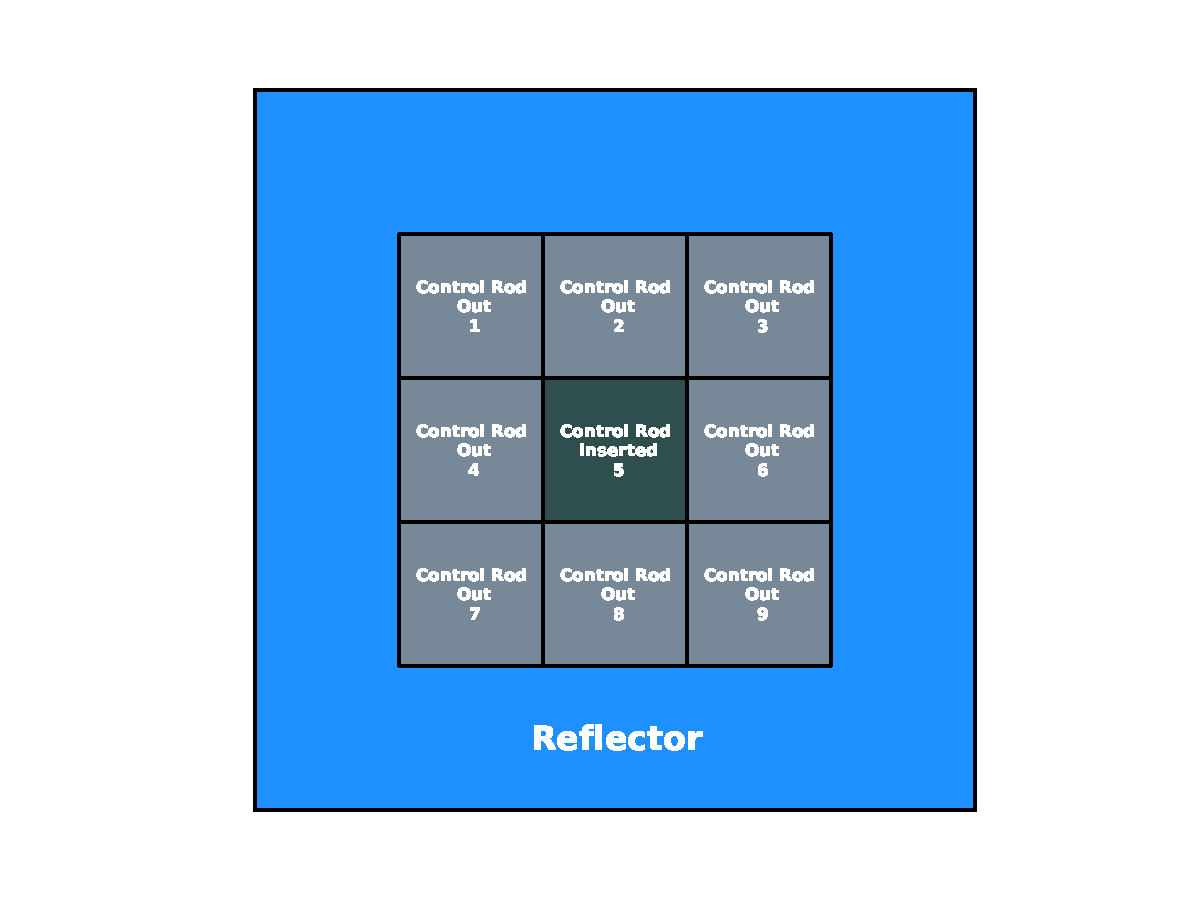
\includegraphics[scale=.75]{./Chapter3/tmi_minicore.pdf}
 \end{center}
\end{figure}  

In order to study the effects of the uncertainties inherent in the few-group cross sections on output parameters of interest in \ac{PARCS}, a few-group covariance matrix is necessary. The few-group covariance matrix is obtained using the 'two-step' method depicted in Fig. \ref{fig:sampler_flow_diagram}. A total of 300 transport calculations with perturbed multigroup cross sections were executed to generate the few-group covariance matrix. In the previous example problems only one output parameter was investigated at a time. However, recall in the discussion of the Smolyak algorithm that interpolation is only performed on the random space. The objective function is evaluated at each abscissa in the random space, returning an output that can still be a function of physical space. In this case the hierarchical surplus is no longer one dimensional. Rather, the hierarchical surplus in Eq. \ref{eq:hierarchical_surplus} is rewritten as,
\begin{equation} 
\label{eq:hierarchical_surplus_space}
   f(\mathbf{x}, x_{j_1}^{i_1},...,x_{j_d}^{i_d}) - 
    A(q-1,d)(\mathbf{x}, x_{j_1}^{i_1},...,x_{j_d}^{i_d})
\end{equation}
where $\mathbf{x} \in \mathcal{D}$ is a coordinate in the spatial domain. When the objective function is a function of spatial coordinates the Smolyak algorithm approximates the function as a linear combination of vectors, the linear weights still being tensor products of basis functions for the random space. To determine the mean and variance of a reduced order model approximation of some space-dependent objective function the $L_2$ norm is taken over the spatial domain $\mathcal{D}$. Similarly, to identify important dimensions using the sensitivity coefficient defined in Eq. \ref{eq:anova_sensitivity} the $L_2$ norm is taken of $\eta_i(\mathbf{x})$.  

The problem in this section considers the core box power distribution of the minicore in Fig. \ref{fig:tmi_minicore} and consequently, the objective function is space dependent. For each simulation in \ac{PARCS} a vector of length nine is returned with each entry containing the relative box power in the fuel assemblies. The box powers are calculated such that the average of all nine entries is identically equal to unity. In the \ac{PARCS} output file the box powers are only given to four digits of accuracy and therefore roundoff error in this problem warrants some attention.  

\subsection{Analysis}
\label{subsec:tmi_analysis}

In this analysis a pure 'two-step' approach is used to compare the results obtained using a reduced order model for the box powers output in \ac{PARCS}. For the 'two-step' approach a few group covariance matrix is constructed and sampled 500 times, with each sample containing perturbed few group cross sections. Each cross section set is propagated through the \ac{PARCS} code and the box powers for the fuel assemblies are extracted from the output file. Ultimately, 500 box power outputs are analyzed statistically to obtain correlations, means, and variances. The same few group covariance matrix is used to sample the reduced order model for the box powers.    

To build a reduced order model, Algorithm \ref{code:rom_algorithm} is applied with a hierarchical surplus threshold of $10^{-4}$ since the \ac{PARCS} box powers are only output to four decimal places. Consequently, roundoff error may accumulate in the fourth decimal point of the reduced order model. A total of 123 executions of \ac{PARCS} were required to construct all single order components of the reduced order model using Clenshaw-Curtis abscissas. Due to the geometry of the \ac{TMI} minicore, 1/8 symmetry is expected in the box power results. Consequently, only fuel assemblies one, four and five are investigated, as defined in Fig. \ref{fig:tmi_minicore}. Sampling results for the mean and standard deviation for the true box power \ac{PARCS} model and the reduced order model are summarized in Tables \ref{table:tmi_mean_sd_mc} and \ref{table:tmi_mean_sd_1d}, respectively. 
%
\begin{table}[!htb] 
\caption{\label{table:tmi_mean_sd_mc} 
Mean and standard deviation data for \ac{TMI} minicore box powers where \ac{PARCS} code is used as objective function. A total of 500 samples were used. Assembly numbers correspond to Fig. \ref{fig:tmi_minicore}.}
\centering
\begin{tabular}{||c|c|c|c|c||} 
\hline \hline
\textbf{Assembly} & \textbf{Mean} & \textbf{99\% CI} & \textbf{Standard Dev.} & \textbf{99\% CI} \\ \hline
1 & 0.8387 & (0.8386, 0.8388) & 0.0007 & (0.0006, 0.0008) \\ \hline 
2 & 1.1499 & (1.1498, 1.1500) & 0.0011 & (0.0010, 0.0012) \\ \hline
3 & 0.8387 & (0.8386, 0.8388) & 0.0007 & (0.0006, 0.0008) \\ \hline
4 & 1.1499 & (1.1498, 1.1500) & 0.0011 & (0.0010, 0.0012) \\ \hline
5 & 1.0453 & (1.0450, 1.0456) & 0.0027 & (0.0025, 0.0029) \\ \hline
6 & 1.1499 & (1.1498, 1.1500) & 0.0011 & (0.0010, 0.0012) \\ \hline
7 & 0.8387 & (0.8386, 0.8388) & 0.0007 & (0.0006, 0.0008) \\ \hline
8 & 1.1499 & (1.1498, 1.1500) & 0.0011 & (0.0010, 0.0012) \\ \hline
9 & 0.8387 & (0.8386, 0.8388) & 0.0007 & (0.0006, 0.0008) \\ 
\hline \hline
\end{tabular}
\end{table}
%
\begin{table}[!htb] 
\caption{\label{table:tmi_mean_sd_1d} 
Mean and standard deviation data for \ac{TMI} minicore box powers where the objective function is a reduced order model for \ac{PARCS} containing only 1D components. A total of 500 samples were used. Assembly numbers correspond to Fig. \ref{fig:tmi_minicore}.}
\centering
\begin{tabular}{||c|c|c|c|c||} 
\hline \hline
\textbf{Assembly} & \textbf{Mean} & \textbf{99\% CI} & \textbf{Standard Dev.} & \textbf{99\% CI} \\ \hline
1 & 0.8387 & (0.8386, 0.8388) & 0.0007 & (0.0006, 0.0008) \\ \hline 
2 & 1.1500 & (1.1499, 1.1501) & 0.0012 & (0.0011, 0.0013) \\ \hline
3 & 0.8387 & (0.8386, 0.8388) & 0.0007 & (0.0006, 0.0008) \\ \hline
4 & 1.1500 & (1.1499, 1.1501) & 0.0012 & (0.0011, 0.0013) \\ \hline
5 & 1.0455 & (1.0452, 1.0458) & 0.0027 & (0.0025, 0.0029) \\ \hline
6 & 1.1500 & (1.1499, 1.1501) & 0.0011 & (0.0010, 0.0012) \\ \hline
7 & 0.8387 & (0.8386, 0.8388) & 0.0007 & (0.0006, 0.0008) \\ \hline
8 & 1.1500 & (1.1499, 1.1501) & 0.0012 & (0.0011, 0.0013) \\ \hline
9 & 0.8387 & (0.8386, 0.8388) & 0.0007 & (0.0006, 0.0008) \\
\hline \hline
\end{tabular}
\end{table}
%
As always, the same random numbers are used to produce each sample when comparing two different methods. The results are identical in all cases to four significant digits and in most cases, to five significant digits. In the reduced order model results notice that the standard deviation for assembly six is slightly off in the fourth decimal place when compared to assemblies two, four, and eight. The standard deviation should be equal in these four assemblies due to symmetry, indicating the presence of roundoff error.        

Adding higher order components in accordance with Algorithm \ref{code:rom_algorithm} did not improve the statistics of the reduced order model. For the purposes of uncertainty quantification the reduced order model consisting entirely of 1D components is sufficient for this problem. The bivariate distributions for the box powers for all combinations of assemblies one, four, and five are given in Fig. \ref{fig:tmi_correlations}.    
\begin{figure}[!htb]
\caption{\label{fig:tmi_correlations}
Multivariate distributions for the box powers of two assemblies. Dashed distributions were obtained by sampling the reduced order model consisting of only 1D components.}
 \begin{center}
  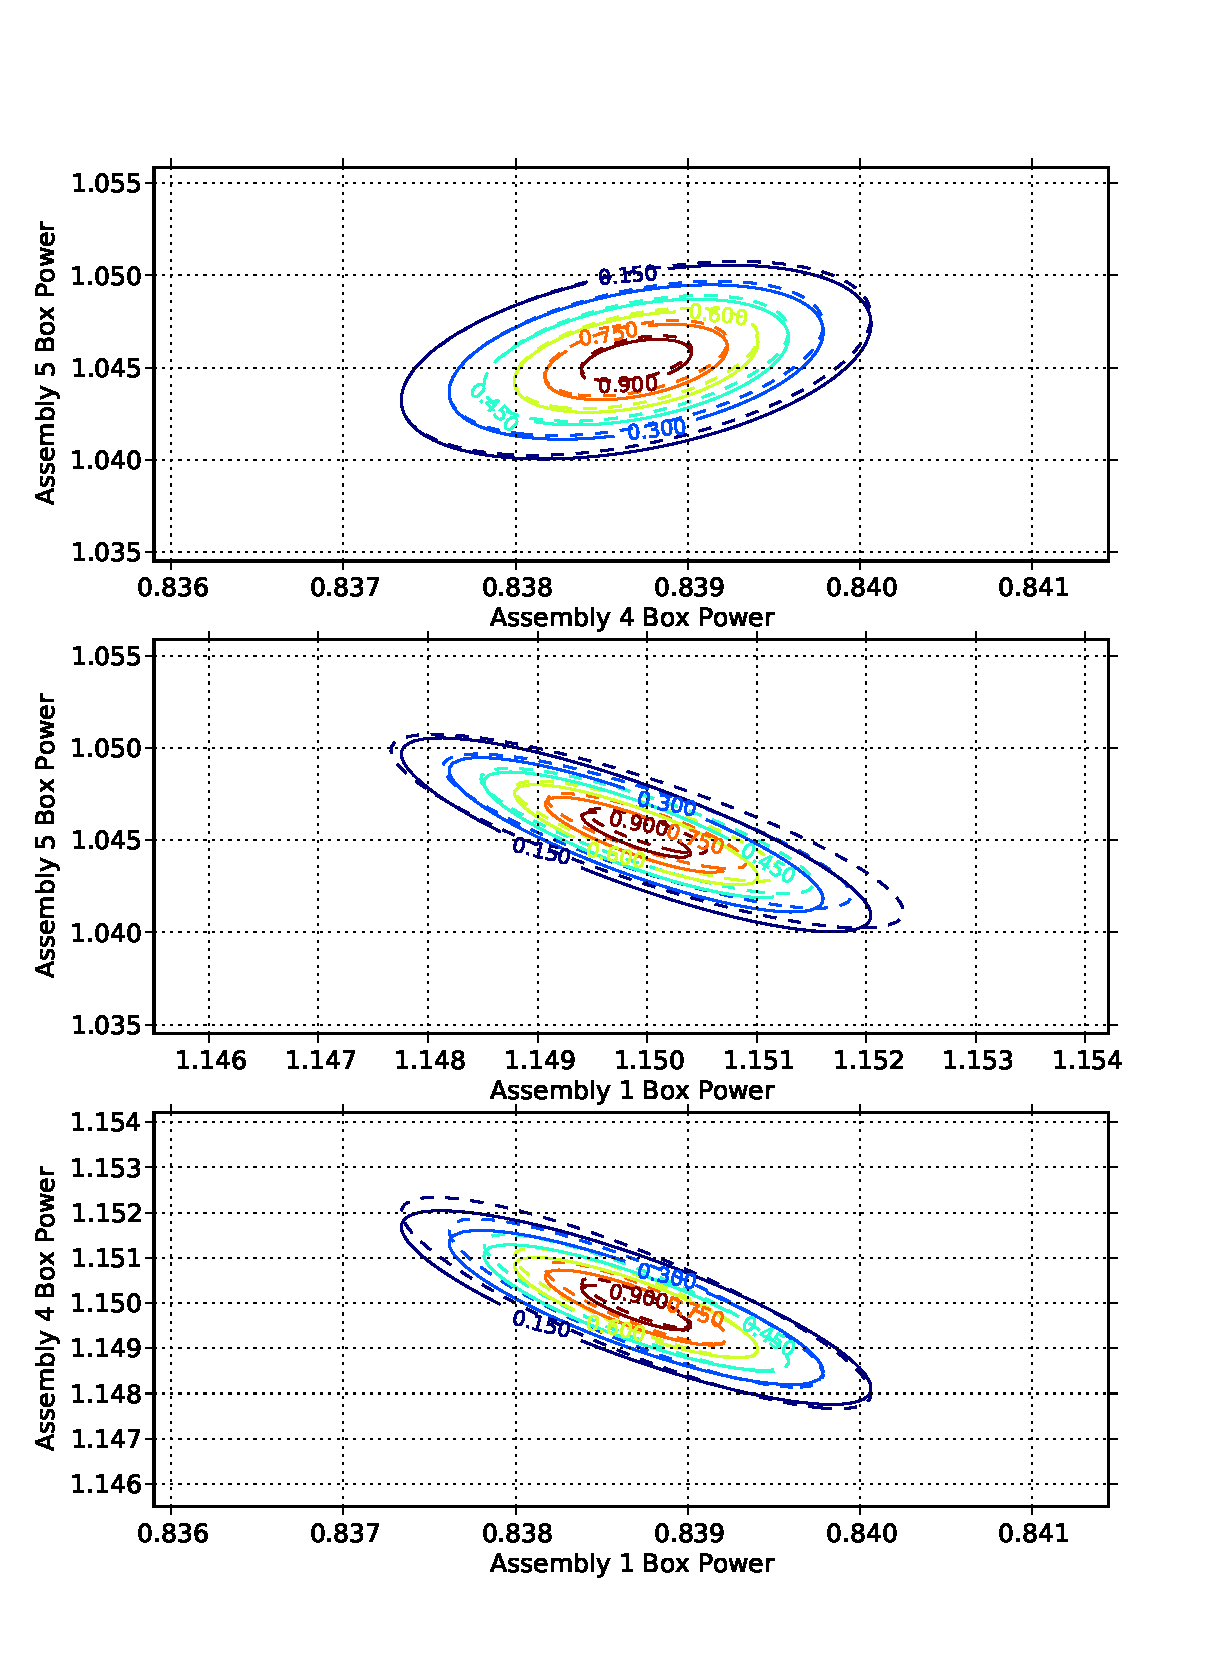
\includegraphics[scale=.70]{./Chapter3/tmi_correlations.pdf}
 \end{center}
\end{figure} 
For each case in Fig. \ref{fig:tmi_correlations} the bivariate distributions are obtained by sampling the reduced order model and \ac{PARCS}. Variations between the overlayed distributions can be attributed to roundoff error. A decrease in the box power of assembly five is equivalent to an increase in the absorption of the assembly's control rods, which effectively shifts the neutron flux away from the central assembly. Consequently, a negative correlation is expected between assemblies one and five and between assemblies one and four. Indeed, statistical sampling has the Pearson correlation coefficient for the box powers of assemblies one and four to be $-0.83$ and $-0.84$ between assemblies one and five. However, negative correlation coefficients between assembly one and assemblies four and five implies a positive correlation coefficient between assemblies four and five. The positive correlation coefficient of $+0.40$ between assemblies four and five is evident in Fig. \ref{fig:tmi_correlations}.  



% General Observations
\section{General Observations}
\label{sec:general_observations}

Before moving on to a large-scale engineering system a few general observations regarding the application of collocation-based and Kriging reduced order models to the uncertainty quantification of the  reactor systems described are in order. Primarily, the demonstration problems indicate that use of only 1D components in the anchored-\ac{ANOVA} expansion provides a very good approximation to the true system under investigation. From a computational point of view, 1D components are cheap to build and their quantity is equal to the number of random variables modeled. Higher order components generally require higher levels of interpolation and so their construction should be minimized if possible. As mentioned in \cite{AHSGC_HighDimensions}, the interaction effects between random variables for most realistic physical systems have a negligible effect on outputs of interest. 

Nevertheless, if multivariate components are needed algorithm \ref{code:rom_algorithm} is able to identify the combination of components most likely to affect the output, which offers significant computational savings. For example, if all components of two random variables were to be included in the anchored-\ac{ANOVA} expansion then 4950 two-dimensional sparse grid interpolants would need to be built. However, if only 5 of the 100 variables are deemed "important" by algorithm \ref{code:rom_algorithm} then only 10 two-dimensional sparse grid interpolants will be built. Not to mention, identification of variables that most affect the variability in some computer code output of interest offers insight into the physical system under consideration. It should be reemphasized that components of the anchored-\ac{ANOVA} used to build reduced order models do not represent the order of effects on the output. Even the 1D component functions can model nonlinear behavior as discussed in section \ref{subsec:anchored_anova}. Rather, the multivariate components describe the effect of input variables upon some output when acting together.    

For the demonstration problems investigated in this chapter, the Clenshaw-Curtis collocation abscissas performed significantly better than Gauss-Patterson. The Clenshaw-Curtis knots offered effectively the same convergence rates as Gauss-Patterson with far fewer function evaluations. Not to mention, Clenshaw-Curtis knots are much easier to generate.

The application of Morris' Algorithm for design variable screening was found to be a visually useful tool for dimension reduction. Whether a computational problem has a large number of dimensions or not the results of Morris' Algorithm can be viewed on a two-dimensional plot. Design variables having the greatest influence on an objective output's behavior become instantly recognizable. After identifying each example problem's key design variables, a reduced order model based on surrogate Kriging was constructed. The Kriging models' ability to reproduce statistics calculated used exact and collocation-based models using only twenty or so basis points demonstrated great promise for further applications.       

However, in all of the example problems analyzed in the current chapter the input uncertainties were calculated systematically beforehand and were therefore relatively small. In other words, engineering judgment never had to be applied in order to estimate the uncertainty of some model input parameter. Uncertainty estimates based on engineering judgment are reasonably expected to be significantly greater than those that can be calculated because more information is known about the latter. The introduction of large uncertainty estimates will be expected in the proceeding application, largely due to the fact that the sources of uncertainty are unknown. Such estimates are expected to negatively impact the smooth construction of surrogate models to represent the applications of interest.          


 



% Bibliography
\bibliographystyle{plain}
\bibliography{./Bibliography/biblio}

\end{document}
